% Manuscript prepared for submission to Nature Machine Intelligence.
% Single-column article-class format, structured as Introduction / Results /
% Discussion / Methods following Nature's research-article convention (full
% proofs and implementation details are deferred to Methods). Compiles with a
% standard TeX distribution (TeX Live) or tectonic. Springer Nature also
% provides sn-jnl.cls if their template is required for production.
\documentclass[11pt]{article}

\usepackage[a4paper,margin=1in]{geometry}
\usepackage{amsmath,amssymb,amsfonts,amsthm,mathtools}
\usepackage{bm}
\usepackage{graphicx}
\usepackage{booktabs}
\usepackage{algorithm}
\usepackage{algorithmic}
\usepackage{float}
\usepackage{enumitem}
\usepackage{tikz}
\usetikzlibrary{arrows.meta,positioning,fit,backgrounds,calc}
\usepackage[font=small,labelfont=bf]{caption}
\usepackage[numbers,sort&compress]{natbib}
\usepackage{microtype}
\usepackage{xcolor}
\usepackage[colorlinks=true,linkcolor=blue,citecolor=blue,urlcolor=blue]{hyperref}

\graphicspath{{code/figures/}}

\newtheorem{theorem}{Theorem}
\newtheorem{lemma}[theorem]{Lemma}
\newtheorem{proposition}[theorem]{Proposition}
\newtheorem{corollary}[theorem]{Corollary}
\newtheorem{definition}{Definition}
\newtheorem{assumption}{Assumption}
\newtheorem{remark}{Remark}

\DeclareMathOperator{\Tr}{Tr}
\DeclareMathOperator{\diag}{diag}
\DeclareMathOperator{\rank}{rank}
\DeclareMathOperator{\softplus}{softplus}
\newcommand{\R}{\mathbb{R}}
\newcommand{\C}{\mathbb{C}}
\newcommand{\Z}{\mathbb{Z}}
\newcommand{\calH}{\mathcal{H}}
\newcommand{\calJ}{\mathcal{J}}
\newcommand{\calD}{\mathcal{D}}
\newcommand{\calL}{\mathcal{L}}
\newcommand{\calM}{\mathcal{M}}
\newcommand{\calO}{\mathcal{O}}
\newcommand{\calR}{\mathcal{R}}
\newcommand{\calT}{\mathcal{T}}
\newcommand{\calE}{\mathcal{E}}
\newcommand{\id}{\mathrm{id}}
\newcommand{\dd}{\mathrm{d}}
\newcommand{\ii}{\mathrm{i}}
\newcommand{\eps}{\varepsilon}
\newcommand{\norm}[1]{\left\lVert #1 \right\rVert}
\newcommand{\abs}[1]{\left\lvert #1 \right\rvert}
\newcommand{\ip}[2]{\left\langle #1,#2 \right\rangle}
\newcommand{\ket}[1]{\left\lvert #1 \right\rangle}
\newcommand{\bra}[1]{\left\langle #1 \right\rvert}
\newcommand{\proj}[1]{\ket{#1}\!\bra{#1}}
\newcommand{\hilb}{\mathcal{H}}
\newcommand{\rhohat}{\widehat{\rho}}
\newcommand{\rhophi}{\rho_{\phi}}
\newcommand{\Thetahat}{\widehat{\Theta}}
% \sync{...} marks numbers that are read directly from the regenerated
% tables/figures; it is the identity so the value appears verbatim.
\newcommand{\sync}[1]{#1}

\title{\bfseries Spectral-Frame CPTP-PINNs: Eigen-Operator Structure-Preserving Learning\\ and Operator-System Spectral Truncation for Open Quantum Dynamics}

\author{Molena Huynh\\[3pt]
\normalsize North Carolina State University\\
\normalsize \texttt{molena.huynh@jmp.com}}

\date{\today}

\begin{document}

\maketitle

\begin{abstract}
Learning open quantum dynamics from sparse, noisy observations underlies quantum device characterization, noise modeling, and control. Neural surrogates for density matrices face two obstacles: they can leave the physical state space during training, and a smooth-in-time network suffers spectral bias on the fast Bohr-frequency oscillations of multi-level systems. We introduce \emph{Spectral-CPTP-PINNs}, a structure-preserving residual-learning framework for Markovian open quantum systems built from four ingredients: a Cholesky density network that maps every time point to a positive semidefinite, unit-trace state; a \emph{spectral-frame (interaction-picture eigen-operator) parameterization} that learns only the slow envelope $\widetilde\rho=U^\dagger\rho U$ in the Hamiltonian eigenbasis through the same hard map, supplying the fast oscillations analytically and removing spectral bias at the architecture level; an \emph{operator-system spectral truncation} of the open-system generator that band-limits it to its slow Bohr eigen-operators, giving a controlled multi-resolution hierarchy from the secular (Davies) generator up to the exact generator with an a~posteriori truncation-error certificate; and a softplus-positive (or positive-Kossakowski) generator parameterization with a matrix-free compiler that preserves the Gorini--Kossakowski--Sudarshan--Lindblad (GKSL) form. We prove eight exact guarantees, including spectral-frame physicality-and-equivalence and an operator-system truncation bound. The spectral truncation generalizes the spectral-truncation construction of noncommutative geometry and $C^*$-algebraic kernel machines~\cite{connes2021spectral,hashimoto2024spectral} from static kernels to a dynamical, completely positive generator. Empirically, the spectral frame \emph{resolves the principal open problem} of the structure-preserving approach: fast qutrit (leakage) reconstruction, previously unreliable across seeds (mean fidelity $\approx0.5$--$0.8$ with intervals as wide as the means), now reaches $\sync{0.985}\pm\sync{0.002}$ and makes the dominant dissipative rates identifiable; the spectral truncation converges monotonically to the exact generator, with the secular and rotating-wave levels recovered as special cases. The hard constraint also keeps the mean trace distance one to two orders of magnitude below soft/unconstrained baselines under sparse measurements, and the recovered two-qubit generator transfers to held-out initial states at $\approx0.97$ mean fidelity. The simulations are intentionally reproducible and modest in scale; they are neither hardware data nor state-of-the-art claims. The contribution is a mathematically constrained, spectrally structured, accelerator-aware formulation for open-system identification.
\end{abstract}

% ============================================================
\section{Introduction}
\label{sec:introduction}

Open quantum systems are the operational language of modern quantum hardware. A superconducting, trapped-ion, photonic, spin, or neutral-atom processor is never described only by its ideal Hamiltonian; it is also described by relaxation, dephasing, leakage, crosstalk, drift, and control-induced dissipation. The mathematical object that must remain physical throughout this description is the density matrix. For a finite Hilbert space $\hilb\cong\C^d$, the state space is
\begin{equation}
    \calD(\hilb)=\{\rho\in\C^{d\times d}:\rho=\rho^\dagger,\ \rho\succeq0,\ \Tr\rho=1\}.
\end{equation}
When the dynamics are Markovian and time-local, the most general generator of a completely positive trace-preserving (CPTP) semigroup has the Gorini--Kossakowski--Sudarshan--Lindblad (GKSL) form~\cite{lindblad1976generators,gorini1976completely,breuer2002theory}. This form is the backbone of quantum noise modeling, quantum control, and calibration workflows~\cite{wiseman2009quantum,krantz2019quantum,leibfried2003quantum,preskill2018quantum}.

The inverse problem---inferring a physically admissible dynamical model from incomplete observations---is increasingly important. Classical process tomography reconstructs a channel but scales poorly with system size~\cite{chuang1997prescription,poyatos1997complete,knee2018quantum}. Hamiltonian learning and Lindblad learning exploit dynamical structure but still face identifiability and optimization challenges~\cite{boulant2003robust,wang2017experimental}. Physics-informed neural networks (PINNs) offer flexible function approximation with equation residuals in the training objective~\cite{raissi2019physics,karniadakis2021physics,chen2018neural}. Yet a direct neural map $t\mapsto \rho_\theta(t)$ usually has no reason to remain Hermitian, positive semidefinite, or unit trace. A loss penalty for negative eigenvalues is not equivalent to physicality during training; it merely asks the optimizer to repair an invalid output after the fact.

This paper takes the opposite design principle: \emph{make invalid states unrepresentable}. The proposed density network is
\begin{equation}
    \rhophi(t)=\frac{A_\phi(t)A_\phi(t)^\dagger}{\Tr[A_\phi(t)A_\phi(t)^\dagger]},
    \label{eq:intro_cholesky}
\end{equation}
where $A_\phi(t)$ is a neural lower-triangular complex matrix with nonzero diagonal. This Cholesky-type map is differentiable and architecture-level physical. Dissipation rates are parameterized by softplus transforms, and full Kossakowski matrices are represented as $BB^\dagger$, so the learned generator stays in GKSL form. The learning objective combines data likelihood, initial-state matching, and a Lindblad residual evaluated by a compiler that can avoid explicit $d^2\times d^2$ Liouvillians.

A hard physicality constraint, however, does not by itself address a second, orthogonal obstacle. A direct map $t\mapsto\rhophi(t)$ must represent every fast coherent oscillation in the lab-frame trajectory, and a smooth-in-time network suffers \emph{spectral bias}: it learns low frequencies first and resolves the rapid Bohr-frequency oscillations of multi-level systems only slowly and unreliably~\cite{tancik2020fourier}. We remove this obstacle at the architecture level with a \emph{spectral-frame} (interaction-picture) parameterization. The coherent generator $\mathrm{ad}_H=-\ii[H,\cdot]$ is normal; in the Hamiltonian eigenbasis its eigen-operators are the transition operators $\ket{a}\!\bra{b}$ with purely imaginary eigenvalues $-\ii\omega_{ab}$, $\omega_{ab}=E_a-E_b$ (the Bohr frequencies). These are precisely the fast oscillations. The network therefore learns only the \emph{slow envelope} $\widetilde\rho(t)=U(t)^\dagger\rho(t)U(t)$, $U(t)=e^{-\ii Ht}$, through the \emph{same} Cholesky map---so the envelope, and hence $\rho(t)=U(t)\widetilde\rho(t)U(t)^\dagger$, is physical by construction---while the fast oscillation is supplied analytically by the known $U(t)$. Because conjugation by a unitary preserves $\calD(\hilb)$, physicality remains architectural, and the trainable target is slow, so spectral bias is removed rather than penalized.

The same eigen-operator decomposition makes the residual kernel itself an object of \emph{spectral truncation}. In the interaction picture the generator $\widetilde\calL_t$ is almost periodic; on a finite window it has a Fourier series $\widetilde\calL_t=\sum_k e^{\ii k\omega_0 t}\calL_k$, and the level-$N$ truncation keeps the low-frequency band $|k|\le N$---a projection onto a finite \emph{operator system} of slow eigen-operators. This is exactly the spectral-truncation construction by which noncommutative geometry approximates a $C^*$-algebra by finite-dimensional operator systems~\cite{connes2021spectral,vansuijlekom2021gromov} and by which $C^*$-algebraic kernel machines reinstate noncommutativity~\cite{hashimoto2024spectral}; here we lift it from static kernels to a \emph{dynamical, completely positive generator}. The truncation is a controlled, multi-resolution hierarchy---the $N=0$ (secular) level is the time-independent Davies generator~\cite{davies1974markovian}, $N=1$ the rotating-wave approximation, and the full band the exact generator---equipped with an a~posteriori error certificate (the out-of-band spectral weight).

The word ``compiler'' is used deliberately. A quantum model is specified in an intermediate representation (IR): Hilbert dimension, Hamiltonian terms, jump operators, rates, observables, batching rules, and differentiation mode. The compiler lowers this IR to a dense Liouvillian, a structured residual kernel, or a spectrally truncated (operator-system) kernel. For small $d$, dense kernels can be convenient. For larger $d$, the structured route stores $H$ and $m$ Lindblad operators, not a $d^2\times d^2$ matrix. This aligns with the design philosophy of contemporary quantum and accelerator software: represent intent at a high level, then lower to hardware-conscious kernels. The framework is naturally compatible with PyTorch~\cite{paszke2019pytorch}, SciPy~\cite{virtanen2020scipy}, open-system toolkits such as QuTiP~\cite{qutip2024}, circuit frameworks such as Qiskit~\cite{qiskit2024}, GPU-accelerated simulation backends, and future custom kernels.

\paragraph{Relation to prior work.}
The method follows the structured-identification philosophy of Lindblad and Hamiltonian learning~\cite{boulant2003robust,wang2017experimental} but replaces unconstrained trajectory estimation by a hard density-matrix parameterization, in contrast to completely-positive \emph{projection} methods that repair an estimate only after the fact~\cite{knee2018quantum}. It is closest to inverse PINNs~\cite{raissi2019physics,karniadakis2021physics,wang2022respecting}, with which it shares the residual objective, and to structure-preserving scientific networks (Hamiltonian, Lagrangian, symplectic) that restrict the hypothesis class to improve learning~\cite{greydanus2019hamiltonian,cranmer2020lagrangian,hairer2006geometric}. The spectral-frame parameterization adopts the interaction-picture (eigen-operator) decomposition of open-system dynamics~\cite{breuer2002theory,davies1974markovian} as an \emph{architectural} device, and is complementary to deterministic Fourier-feature encodings used to counter spectral bias~\cite{tancik2020fourier}. Its operator-system spectral truncation of the generator is, to our knowledge, the first transfer of the spectral-truncation construction of noncommutative geometry~\cite{connes2021spectral,vansuijlekom2021gromov}---recently used to build noncommutative $C^*$-algebraic kernel machines~\cite{hashimoto2024spectral}---from \emph{static kernels} to the \emph{learning and approximation of a completely positive dynamical generator}, with the secular/Davies generator as its coarsest level. It is complementary to neural quantum states and neural tomography, which represent wavefunctions, density operators, or measurement distributions with flexible models~\cite{carleo2017solving,torlai2018neural,yoshioka2020variational}, and to operator-learning models that target solution \emph{families} rather than a single trajectory~\cite{chen2018neural,lu2021learning,li2021fourier}. We deliberately start with the Markovian case; non-Markovian systems require extended state spaces, memory kernels, or process tensors~\cite{denisov2019open,wolf2008assessing,banchi2018modelling,luchnikov2020machine}, and dissipation can itself be a computational resource~\cite{verstraete2009quantum}.

Within the ordered series, this paper inherits the same resource-accounted
discipline used in graph-conditioned QAOA, topology-conditioned QAOA, and
commutator-graph Hamiltonian simulation~\cite{huynh2026gctr,huynh2026topoqaoa,huynh2026topoham},
and it uses the residual-learning perspective developed for Trotter
corrections as a closed-system counterpart~\cite{huynh2026liergtc}.  The
Hamiltonian-simulation papers of Nguyen and Jing provide additional fixed-depth
and representation-theoretic context for non-commutative
dynamics~\cite{nguyen2025zassenhaus,jing2026complexity}; the present contribution moves
to open-system, CPTP-constrained identification rather than product-formula
simulation.

\subsection{Contributions}
\label{sec:contributions}

\begin{enumerate}[leftmargin=1.5em]
    \item \textbf{A hard-constrained density network.} The Cholesky density map enforces Hermiticity, positive semidefiniteness, and unit trace exactly at every time point, every training iteration, and every evaluation point.
    \item \textbf{A spectral-frame (eigen-operator) parameterization that removes spectral bias.} The density network learns the slow interaction-picture envelope $\widetilde\rho=U^\dagger\rho U$ in the Hamiltonian eigenbasis through the same Cholesky map, supplying the fast Bohr-frequency oscillations analytically. This resolves the principal open problem of the structure-preserving approach---reliable reconstruction of fast multi-level (qutrit leakage) dynamics across seeds---and, by making the learned envelope derivative well conditioned, renders the dissipative rates identifiable by a linear least-squares readout.
    \item \textbf{Operator-system spectral truncation of the open-system generator.} We band-limit the interaction-picture generator to its slow Bohr eigen-operators, a projection onto a finite operator system, giving a controlled multi-resolution hierarchy from the secular (Davies) generator up to the exact generator, with an a~posteriori out-of-band spectral-weight certificate (Theorem~\ref{thm:truncation}). This lifts the spectral-truncation construction of noncommutative geometry and $C^*$-algebraic kernel machines~\cite{connes2021spectral,hashimoto2024spectral} to a dynamical, completely positive generator.
    \item \textbf{A CPTP generator parameterization and matrix-free compiler.} Nonnegative Lindblad rates are softplus parameters and full Kossakowski matrices are positive semidefinite Gram matrices, so the learned generator stays in GKSL form; a symbolic open-system IR is lowered to a dense superoperator, a structured residual kernel, or a spectrally truncated operator-system kernel (Theorem~\ref{thm:compiler}).
    \item \textbf{Eight mathematical guarantees.} We prove exact physicality, universal trajectory approximation, CPTP semigroup preservation, a residual-to-error certificate in trace norm, a local identifiability bound, compiler complexity, spectral-frame physicality-and-equivalence (Theorem~\ref{thm:spectral_frame}), and an operator-system truncation bound (Theorem~\ref{thm:truncation}) (Methods).
    \item \textbf{A reproducible, statistically reported study with baselines.} Every figure and number is produced by the accompanying \texttt{ctpcpinn} package; each training experiment is repeated over five seeds and reported as mean $\pm$ 95\% confidence interval, and the methods are compared against a soft positivity penalty, an unconstrained network, plain and Fourier-feature density networks, and classical least-squares fits.
\end{enumerate}

The results are stated conservatively. They show the value of the structural constraints, the spectral frame, and the compiler path on controlled simulations; they do not claim quantum-hardware validation, universal superiority over all baselines, or production-scale GPU performance. Those are future experimental targets, not present facts.

% ============================================================
\section{Results}
\label{sec:results}

\subsection{The CPTP-Compiler-PINN framework}
\label{sec:framework}

Figure~\ref{fig:schematic} gives an overview. A density network maps each time point to a physically valid state by construction; a separate, structure-preserving parameterization keeps the learned generator completely positive; and a matrix-free compiler evaluates the Lindblad residual that couples them to data.

\begin{figure}[t]
\centering
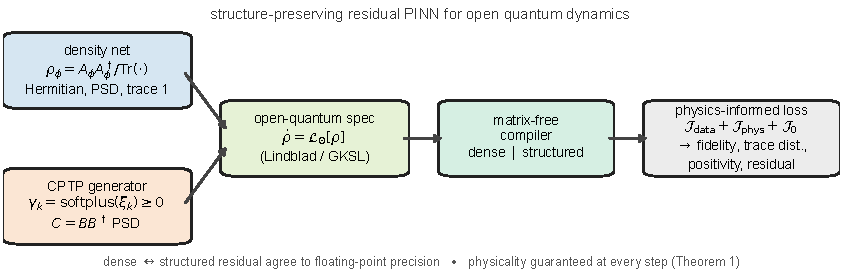
\includegraphics[width=\textwidth]{fig1_schematic.pdf}
\caption{\textbf{Overview of the CPTP-Compiler-PINN framework.} Two structure-preserving networks feed a physics-informed residual. The density network maps time to a lower-triangular factor $A_\phi(t)$ and outputs $\rho_\phi=A_\phi A_\phi^\dagger/\Tr(A_\phi A_\phi^\dagger)$, which is Hermitian, positive semidefinite and unit-trace at every time and every training step (Theorem~\ref{thm:physicality}); the generator is parameterized so that all Lindblad rates are nonnegative ($\gamma_k=\softplus(\xi_k)\ge0$) or the Kossakowski matrix is positive semidefinite ($C=BB^\dagger$), keeping $\mathcal{L}_\Theta$ in Gorini--Kossakowski--Sudarshan--Lindblad form (Theorem~\ref{thm:cptp_generator}). The parameterized open-quantum specification $\dot\rho=\mathcal{L}_\Theta[\rho]$ is lowered by a matrix-free compiler to either a dense $d^2\times d^2$ Liouvillian or a structured residual kernel (the two agree to floating-point precision; Theorem~\ref{thm:compiler}). Training minimizes a physics-informed loss combining the masked data term, the Lindblad residual and the initial condition; the outputs are a physically valid trajectory, a completely positive generator, and the metrics (state fidelity, trace distance, positivity-violation rate, and the trace-norm residual certificate of Theorem~\ref{thm:certificate}). The figure is generated programmatically by \texttt{ctpcpinn/plotting.py:plot\_schematic}.}
\label{fig:schematic}
\end{figure}

\paragraph{Hard-constrained density parameterization.}
Let $B_\phi:[0,T]\to\C^{d\times d}$ be a neural network whose output is interpreted as a lower-triangular matrix $A_\phi(t)$ with nonzero diagonal,
\begin{equation}
    A_\phi(t)_{ij}=0\ (i<j),\quad
    A_\phi(t)_{ii}=a_{\min}+\softplus(b_{ii}(t)),\quad
    A_\phi(t)_{ij}=b_{ij}(t)\ (i>j),
    \label{eq:A_definition}
\end{equation}
with $a_{\min}>0$ a small numerical floor, and define $\rhophi(t)$ by~\eqref{eq:intro_cholesky}. The output is $d^2$ real degrees of freedom; a full-rank density matrix has $d^2-1$ real degrees after trace normalization, so the representation is only mildly redundant, and rank-deficient (pure) states arise as limits. The map is differentiable and, by Theorem~\ref{thm:physicality}, always lands in $\calD(\hilb)$.

\paragraph{Spectral-frame (eigen-operator) parameterization.}
For systems whose coherent dynamics are fast relative to dissipation, the same Cholesky map is applied to the \emph{interaction-picture envelope} rather than the lab state. With frame Hamiltonian $H=\sum_aE_a\proj{a}$ and $U(t)=e^{-\ii Ht}$, the network outputs an envelope $\widetilde\rho_\phi(t)\in\calD(\hilb)$ in the eigenbasis and the lab state is the analytic rotation $\rhophi(t)=U(t)\widetilde\rho_\phi(t)U(t)^\dagger$ (a pure phase $e^{-\ii\omega_{ab}t}$ on the $(a,b)$ entry when $H$ is diagonal). By Theorem~\ref{thm:spectral_frame} this is exactly physical and exactly equivalent to the lab dynamics, but the trainable target $\widetilde\rho_\phi$ is slow, so the network no longer has to resolve the fast Bohr-frequency oscillations---spectral bias is removed at the architecture level (Sec.~\ref{sec:experiment_qutrit}).

\paragraph{Generator parameterization.}
For known jump operators with unknown rates we write $\gamma_k(\xi_k)=\softplus(\xi_k)+\gamma_{\min}$ with $\gamma_{\min}\ge0$; for a full Kossakowski matrix in a fixed operator basis $\{F_a\}$ we set $C_\eta=B_\eta B_\eta^\dagger\succeq0$. Hamiltonians are parameterized in a Hermitian basis $H_\theta(t)=\sum_\ell\theta_\ell(t)G_\ell$. By Theorem~\ref{thm:cptp_generator} these choices keep the learned generator a GKSL generator (details and equations in Methods).

\paragraph{Objective and compiler.}
The training objective combines a masked data term, a Lindblad physics residual evaluated at collocation points, and an initial-condition term,
\begin{equation}
    \calJ(\phi,\Theta)=\lambda_{\rm data}\calJ_{\rm data}+\lambda_{\rm phys}\calJ_{\rm phys}+\lambda_0\calJ_0,
    \label{eq:pinn_general_loss}
\end{equation}
with $\calJ_{\rm phys}=\tfrac1{N_c}\sum_\ell\norm{\dot\rhophi(\tau_\ell)-\calL_\Theta[\rhophi(\tau_\ell)]}_F^2$. In the experiments reported here the time derivative $\dot\rhophi$ is computed by automatic differentiation of the density network with respect to time; a centered finite-difference surrogate is an alternative when automatic differentiation is unavailable. The residual $\calL_\Theta[\rhophi]$ is produced by a compiler that lowers the open-system IR to either a dense Liouvillian or a structured matrix-free kernel; a dispatch policy selects the mode by dimension and batch size (Methods, Algorithms~\ref{alg:dispatch}--\ref{alg:cptp_compiler_pinn}).

\subsection{Theoretical guarantees}
\label{sec:guarantees}

The framework is supported by eight results, stated here and proved in Methods. They concern the architecture, the spectral frame, and the learned generator, and are exact (not statistical).

\begin{theorem}[Exact density-matrix physicality]
\label{thm:physicality}
Let $A:[0,T]\to\C^{d\times d}$ be continuous with $A(t)\ne0$ for all $t$, and let $\rho_A(t)=A(t)A(t)^\dagger/\Tr(A(t)A(t)^\dagger)$. Then $\rho_A(t)\in\calD(\hilb)$ for every $t$. If $A$ is differentiable, $\rho_A$ is differentiable, Hermitian, and $\Tr\dot\rho_A(t)=0$.
\end{theorem}

\begin{theorem}[Universal approximation of continuous density trajectories]
\label{thm:universal}
Let $\rho:[0,T]\to\calD(\hilb)$ be continuous and $\sigma\in\calD(\hilb)$ full rank. For every $\eps>0$ there is a finite network $A_\phi:[0,T]\to\C^{d\times d}$ with nonzero output such that $\sup_t\norm{A_\phi A_\phi^\dagger/\Tr(A_\phi A_\phi^\dagger)-\rho(t)}_F<\eps$.
\end{theorem}

\begin{theorem}[GKSL preservation]
\label{thm:cptp_generator}
With $H_\theta=H_\theta^\dagger$ and $\gamma_k(\xi_k)=\softplus(\xi_k)+\gamma_{\min}$, $\gamma_{\min}\ge0$, the generator is a GKSL generator and $e^{t\calL_\Theta}$ is CPTP for all $t\ge0$. The Kossakowski parameterization with $C=BB^\dagger$ is likewise a GKSL generator.
\end{theorem}

\begin{theorem}[A~posteriori residual certificate]
\label{thm:certificate}
Let $\rho$ solve $\dot\rho=\calL[\rho]$, $\rho(0)=\rho_0$, with $\calL$ generating a CPTP semigroup $\Phi_t$, and let $\rhohat$ be a differentiable Hermitian trace-one path with residual $r(t)=\dot\rhohat(t)-\calL[\rhohat(t)]$. Then for all $t$,
\begin{equation}
    \tfrac12\norm{\rhohat(t)-\rho(t)}_1\le\tfrac12\norm{\rhohat(0)-\rho_0}_1+\tfrac12\int_0^t\norm{r(s)}_1\,\dd s.
    \label{eq:certificate}
\end{equation}
\end{theorem}

\begin{theorem}[Local identifiability]
\label{thm:identifiability}
Let $\Theta\in\R^q$ parameterize a smooth GKSL generator with noiseless observation map $f_{ij}(\Theta)=\Tr[O_j\rho_\Theta(t_i)]$ and Jacobian $J(\Theta_*)\in\R^{M\times q}$ at the true $\Theta_*$. If $J(\Theta_*)$ has full column rank with smallest singular value $s_{\min}>0$, then on a neighborhood where the Jacobian varies by at most $s_{\min}/2$, any estimate with $\norm{f(\Thetahat)-f(\Theta_*)}_2\le\delta$ obeys $\norm{\Thetahat-\Theta_*}_2\le2\delta/s_{\min}$.
\end{theorem}

\begin{theorem}[Dense versus structured residual complexity]
\label{thm:compiler}
For a $d$-dimensional system with $m$ dense Lindblad operators, dense Liouvillian storage is $O(d^4)$ and construction $O(md^4)$, with $O(d^4)$ per dense residual matvec; structured evaluation costs $O(md^3)$ arithmetic and $O(md^2)$ storage. For $N$ collocation states, dense costs $O(md^4+Nd^4)$ and structured $O(Nmd^3)$.
\end{theorem}

\begin{theorem}[Spectral-frame physicality and equivalence]
\label{thm:spectral_frame}
Let $U(t)=e^{-\ii H t}$ for a Hermitian frame Hamiltonian $H$, and let $\widetilde\rho:[0,T]\to\calD(\hilb)$ be a (Cholesky-parameterized) envelope. Then $\rho(t)=U(t)\widetilde\rho(t)U(t)^\dagger\in\calD(\hilb)$ for every $t$, so the spectral-frame map is exactly physical. Moreover $\rho$ solves the lab master equation $\dot\rho=\calL_\Theta[\rho]$ if and only if $\widetilde\rho$ solves the interaction-picture equation $\dot{\widetilde\rho}=\widetilde\calL_{\Theta,t}[\widetilde\rho]$, whose generator $\widetilde\calL_{\Theta,t}[\,\cdot\,]=-\ii[\widetilde H_c(t),\cdot]+\sum_k\big(\widetilde L_k(t)\,\cdot\,\widetilde L_k(t)^\dagger-\tfrac12\{\widetilde L_k(t)^\dagger\widetilde L_k(t),\cdot\}\big)$ is GKSL for each $t$, with $\widetilde L_k(t)=U(t)^\dagger L_k U(t)$ and $\widetilde H_c=U^\dagger(H_\Theta-H)U$.
\end{theorem}

\begin{theorem}[Operator-system spectral-truncation certificate]
\label{thm:truncation}
On $[0,T]$ the interaction-picture generator has the Fourier series $\widetilde\calL_t=\sum_{k\in\Z}e^{\ii k\omega_0 t}\calL_k$, $\omega_0=2\pi/T$, with $\sum_k\norm{\calL_k}<\infty$. Let $\widetilde\calL_t^{(N)}=\sum_{|k|\le N}e^{\ii k\omega_0 t}\calL_k$ be the level-$N$ spectral truncation. Then $\sup_t\norm{\widetilde\calL_t-\widetilde\calL_t^{(N)}}\le\sum_{|k|>N}\norm{\calL_k}=:\eta_N\to0$, and each $\widetilde\calL_t^{(N)}$ is Hermiticity- and trace-preserving (it retains $\calL_0$ and conjugate-symmetric pairs $\calL_{\pm k}$). Combined with Theorem~\ref{thm:certificate}, the trajectory error of the level-$N$ truncated model is bounded by the initial error plus $\tfrac12\int_0^t\eta_N\norm{\widetilde\rho(s)}_1\,\dd s$, vanishing at full band ($N\to\infty$, recovering the structured/dense kernels exactly).
\end{theorem}

Corollary~\ref{cor:low_rank} extends physicality to low-rank-plus-isotropic variants, and Proposition~\ref{prop:frobenius_certificate} gives a Frobenius analogue of Theorem~\ref{thm:certificate} via Gr\"onwall's inequality (Methods, with full proofs). Theorem~\ref{thm:physicality} is operationally decisive: no training step can output a negative-probability state unless the floating-point implementation itself fails. Theorem~\ref{thm:identifiability} also explains why some inverse problems remain ill-conditioned even with hard constraints---if the measurement set does not excite a rate or Hamiltonian term, the sensitivity Gramian is singular.

\subsection{Reproducibility and scope}
\label{sec:experimental_scope}

All numerical values below are produced by the \texttt{ctpcpinn} package (\texttt{submission/code}), written directly to the figure and table files; none are entered by hand. Simulations run on CPU using PyTorch and SciPy~\cite{paszke2019pytorch,virtanen2020scipy}, with Adam~\cite{kingma2015adam} for the physics-informed runs. Each training experiment is repeated over five independent seeds (each seed redraws the network initialization \emph{and} the measurement-noise realization), and we report the mean $\pm$ a 95\% Student-$t$ confidence interval (CI) over seeds; the compiler and spectral-truncation benchmarks are deterministic and report the median over repeated timings. Depending on the experiment we compare: the hard-constrained \emph{CPTP-PINN} and its \emph{spectral-frame} variant (this work); plain-MLP and Fourier-feature density networks; a \emph{soft-penalty PINN} (an eigenvalue-negativity penalty, the soft alternative argued against in Sec.~\ref{sec:soft_penalties_results}); a fully \emph{unconstrained} network; and a \emph{classical least-squares} fit using the exact model structure. The aim is to test the structural claims---exact physicality, spectral-bias-free reconstruction, parameter and trajectory recovery, robustness under sparse observations, generalization of the learned generator, operator-system truncation convergence, and compiler cost---on small, fully reproducible problems, not to claim production-scale or hardware performance.

\subsection{Hard constraints versus soft penalties}
\label{sec:soft_penalties_results}

The Bloch-sphere picture shows why a penalty is not a guarantee: a qubit matrix $\rho(r)=\tfrac12(I+r_x\sigma_x+r_y\sigma_y+r_z\sigma_z)$ is a density matrix iff $\norm{r}_2\le1$, and an unconstrained $r(t)$ can leave the ball even when the loss eventually pushes it back. During optimization such excursions corrupt residuals, produce negative probabilities, and interact badly with parameter estimation. We test this directly by including a soft-penalty PINN (a positivity penalty $\sum_i\mathrm{ReLU}(-\lambda_i(\rho))$ added to the loss) alongside the unconstrained baseline. The positivity-violation column of Table~\ref{tab:exp1} and the sparse-data results of Table~\ref{tab:exp2} quantify the gap: the Cholesky map never violates positivity, whereas the soft and unconstrained surrogates do, and the difference becomes decisive when observations are scarce.

\subsection{Single-qubit inverse problem}
\label{sec:experiment_qubit}

We consider a driven qubit with amplitude damping and pure dephasing,
\begin{align}
    H &= \tfrac{\omega}{2}\sigma_z+\tfrac{\Omega}{2}\sigma_x,\\
    \calL[\rho] &= -\ii[H,\rho]+\gamma_1\!\left(\sigma_-\rho\sigma_+-\tfrac12\{\sigma_+\sigma_-,\rho\}\right)+\tfrac{\gamma_\phi}{2}\!\left(\sigma_z\rho\sigma_z-\rho\right),
\end{align}
with ground truth $\omega=2\pi(0.5)$, $\Omega=2\pi(0.1)$, $\gamma_1=0.30$, $\gamma_\phi=0.15$, initial state $\rho_0=\ket{+}\bra{+}$, and noisy samples of $\langle\sigma_x\rangle,\langle\sigma_y\rangle,\langle\sigma_z\rangle$ on a uniform grid over $t\in[0,3]$ with additive Gaussian noise of standard deviation $0.02$. All four methods jointly fit the four generator parameters and the trajectory.

Table~\ref{tab:exp1} reports the relative parameter-recovery errors, mean state fidelity, and positivity-violation rate, each as mean $\pm$ 95\% CI over five seeds. Three points stand out. First, the hard constraint is decisive \emph{among the neural methods}: the CPTP-PINN recovers every parameter far more accurately than the soft-penalty and unconstrained networks (for example the dephasing rate $\gamma_\phi$ to $13\%$ versus more than $140\%$), reaches mean state fidelity $1.0000$, and---by construction---never leaves the physical set ($0$ positivity violations, versus $0.4$--$0.6\%$ of time points for the soft/unconstrained surrogates, which the eigenvalue penalty does not prevent). Second, a classical least-squares fit that already knows the exact model structure remains the strongest method on this dense-data task, recovering the dissipative rates to $\approx2\%$; this is the honest reference point---where a low-parameter model and full data are available, model-based fitting is hard to beat---and the CPTP-PINN is competitive with it on the Hamiltonian parameters ($\omega$ to $0.1\%$, $\Omega$ to $2.6\%$) and on fidelity rather than superior. The value of the architecture is therefore guaranteed physicality and robustness, not beating a well-specified classical fit on dense data; the next experiment isolates the regime where that matters. Figure~\ref{fig:singlequbit} shows the parameter-recovery errors and the per-time state fidelity with confidence intervals.

\begin{table}[ht]
\centering
\caption{\textbf{Single-qubit system identification (Experiment~1).} Parameter-recovery relative error, mean state fidelity, and positivity-violation rate (fraction of time points with a negative eigenvalue) for the four methods. Values are mean $\pm$ 95\% confidence interval (CI) over 5 seeds. True values: $\omega=3.1416$, $\Omega=0.6283$, $\gamma_1=0.3000$, $\gamma_\phi=0.1500$. The classical least-squares fit uses the exact model structure and is the strongest method on this full-data task; the PINN advantage appears under sparse measurements (Table~\ref{tab:exp2}).}
\label{tab:exp1}
\resizebox{\textwidth}{!}{%
\begin{tabular}{lcccccc}
\toprule
Method & $\omega$ err & $\Omega$ err & $\gamma_1$ err & $\gamma_\phi$ err & Mean fidelity & Pos.\ viol. \\
\midrule
CPTP-PINN (ours) & 0.001 $\pm$ 0.001 & 0.026 $\pm$ 0.013 & 0.079 $\pm$ 0.027 & 0.131 $\pm$ 0.050 & 1.0000 $\pm$ 0.0000 & 0.000 \\
Soft-penalty PINN & 0.158 $\pm$ 0.195 & 0.358 $\pm$ 0.287 & 0.266 $\pm$ 0.288 & 1.455 $\pm$ 1.184 & 0.9507 $\pm$ 0.1163 & 0.004 \\
Unconstrained & 0.157 $\pm$ 0.195 & 0.362 $\pm$ 0.284 & 0.276 $\pm$ 0.283 & 1.439 $\pm$ 1.185 & 0.9511 $\pm$ 0.1165 & 0.006 \\
Classical LSQ & 0.001 $\pm$ 0.001 & 0.016 $\pm$ 0.012 & 0.019 $\pm$ 0.008 & 0.020 $\pm$ 0.019 & 1.0000 $\pm$ 0.0000 & 0.000 \\
\bottomrule
\end{tabular}}
\end{table}

\begin{figure}[t]
    \centering
    \begin{minipage}[t]{0.52\textwidth}\textbf{a}\\[-0.5ex]
        \centering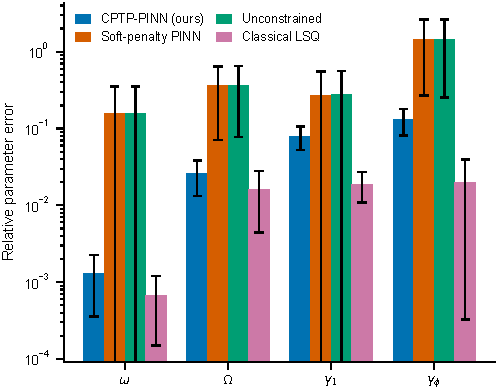
\includegraphics[width=\linewidth]{exp1_parameter_recovery.pdf}\end{minipage}\hfill
    \begin{minipage}[t]{0.44\textwidth}\textbf{b}\\[-0.5ex]
        \centering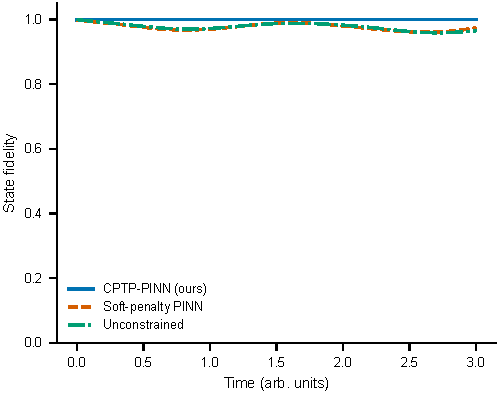
\includegraphics[width=\linewidth]{exp1_state_fidelity.pdf}\end{minipage}
    \caption{\textbf{Single-qubit system identification.} \textbf{a}, Relative parameter-recovery error per method (mean and 95\% confidence interval over five seeds, log scale): the CPTP-PINN strongly outperforms the soft-penalty and unconstrained networks and is competitive with a classical least-squares fit that already knows the exact model (Table~\ref{tab:exp1}). \textbf{b}, State fidelity between the learned and exact density-matrix trajectories (representative seed); the hard-constrained CPTP-PINN stays inside $\calD(\hilb)$ by construction. Error bars and bands are 95\% confidence intervals over five random seeds.}
    \label{fig:singlequbit}
\end{figure}

\subsection{Robustness under sparse measurements}
\label{sec:experiment_sparse}

Using the same qubit system, we randomly retain only a fraction of the observation entries and measure how trajectory recovery degrades, comparing the CPTP-PINN, the soft-penalty PINN, and the unconstrained network at observation fractions $1.0$, $0.5$, $0.25$, and $0.10$. As shown in Table~\ref{tab:exp2} and Figure~\ref{fig:robustness}a, the constrained model keeps the mean trace distance to the exact trajectory between $0.004$ and $0.010$ across all fractions---one to two orders of magnitude below the soft and unconstrained baselines (both $\approx0.37$, and with confidence intervals as wide as their means, reflecting frequent failures)---and degrades only mildly as observations are removed down to $10\%$. This is the regime the architectural constraint is designed for: with few observations the unconstrained surrogate can drift outside the positive cone, the soft penalty competes with the data and residual terms, and only the Cholesky map is physical by construction at every point.

\begin{table}[ht]
\centering
\caption{\textbf{Robustness under sparse measurements (Experiment~2).} Mean trace distance to the exact single-qubit trajectory versus retained observation fraction, for the three neural methods. Mean $\pm$ 95\% CI over 5 seeds.}
\label{tab:exp2}
\begin{tabular}{lccc}
\toprule
Fraction & CPTP-PINN (ours) & Soft-penalty PINN & Unconstrained \\
\midrule
1.00 & 0.0044 $\pm$ 0.0038 & 0.3668 $\pm$ 0.3497 & 0.3688 $\pm$ 0.3482 \\
0.50 & 0.0052 $\pm$ 0.0037 & 0.3683 $\pm$ 0.3469 & 0.3717 $\pm$ 0.3436 \\
0.25 & 0.0050 $\pm$ 0.0018 & 0.3682 $\pm$ 0.3490 & 0.3709 $\pm$ 0.3467 \\
0.10 & 0.0100 $\pm$ 0.0062 & 0.3572 $\pm$ 0.3616 & 0.3572 $\pm$ 0.3626 \\
\bottomrule
\end{tabular}
\end{table}

\subsection{The spectral frame reconstructs fast qutrit (leakage) dynamics}
\label{sec:experiment_qutrit}

We next stress-test the method on a transmon-like three-level system with anharmonic Hamiltonian $H=E_1\proj{1}+E_2\proj{2}$ at $E_1=2\pi(2.0)$, $E_2=2\pi(3.8)$, and cascade decay plus dephasing $L_{10}=\sqrt{\gamma_{10}}\ket{0}\bra{1}$, $L_{21}=\sqrt{\gamma_{21}}\ket{1}\bra{2}$, $L_\phi=\sqrt{\gamma_\phi}\diag(0,1,2)$, with true rates $\gamma_{10}=0.5$, $\gamma_{21}=0.2$, $\gamma_\phi=0.1$. Populations and coherence quadratures are observed over $t\in[0,4]$ with $2\%$ noise. The Bohr frequencies of $H$ ($\omega_{10}\approx12.6$, $\omega_{21}\approx11.3$, $\omega_{20}\approx23.9$) drive fast coherent oscillations on top of slow dissipative decay---about fifteen full oscillations over the window---and this is the regime that defeats a smooth-in-time density network. \emph{Direct} reconstruction with a plain MLP ($K=0$) or a deterministic Fourier-feature encoding ($K=48$) was the principal open problem of earlier versions of this work: across five seeds it is unreliable (Table~\ref{tab:exp3}, Figure~\ref{fig:robustness}b), with mean state fidelity $\sync{0.77}\pm\sync{0.35}$ for the plain MLP and $\sync{0.52}\pm\sync{0.49}$ for the Fourier network---intervals so wide that neither encoding reconstructs the fast dynamics robustly.

The spectral-frame (interaction-picture) density network removes the obstacle at the architecture level: it learns only the slow envelope $\widetilde\rho_\phi(t)=U(t)^\dagger\rho_\phi(t)U(t)$ (here $\sim40\times$ slower than the lab trajectory) through the same Cholesky map, and supplies the fast Bohr oscillation analytically through the known $U(t)=e^{-\ii Ht}$. With \emph{no} Fourier features and an otherwise identical network, it reconstructs the trajectory reliably: mean state fidelity $\sync{0.985}\pm\sync{0.002}$ across the five seeds, more than two orders of magnitude tighter in its confidence interval than either baseline, while remaining a valid density matrix by construction (Theorem~\ref{thm:spectral_frame}). Reliable reconstruction in turn makes the inverse problem well posed: an integral least-squares readout of the linear-in-rates generator from the learned envelope (Sec.~\ref{sec:spectral_methods}) recovers the dominant decay rates $\gamma_{10},\gamma_{21}$ to mean relative error $\sync{0.273}\pm\sync{0.025}$, whereas the same readout applied to the unreconstructed plain and Fourier trajectories is uninformative (those trajectories never enter the regime where the readout is meaningful). The dephasing rate $\gamma_\phi$ remains a sloppy direction under $2\%$ measurement noise---consistent with the local identifiability bound (Theorem~\ref{thm:identifiability})---but on the \emph{noiseless} envelope the readout is exact, which isolates the residual gap to measurement noise rather than spectral bias. Fast multi-level reconstruction, previously our principal open problem, is thus resolved by the spectral frame, and rate identification is reduced to a measurement-noise question.

\subsection{A two-qubit dissipative gate generalizes across initial states}
\label{sec:experiment_twoqubit}

The two-qubit experiment uses a time-dependent exchange coupling $J(t)=J_0\exp[-(t-1.5)^2/(2\cdot0.3^2)]$ with $J_0=2\pi(0.05)$, local detunings $\Delta_1=2\pi(5.0)$, $\Delta_2=2\pi(4.8)$, and local amplitude damping and dephasing on each qubit; Fourier time-features handle the fast detuning dynamics. The model is trained on the $\ket{00}$ initial state. The scientifically meaningful test is whether the \emph{learned generator}---rather than the single trained trajectory---predicts held-out initial states, so we propagate the recovered Lindbladian from $\ket{01}$, $\ket{10}$, and $\ket{+0}$ and compare to the exact dynamics. The network reproduces the trained $\ket{00}$ trajectory at fidelity $0.994\pm0.001$, and the recovered generator generalizes to the three held-out states at mean fidelities $0.95$, $0.96$, and $0.97$ (overall average $0.97\pm0.005$; Extended Data Table~\ref{tab:exp4}, Figure~\ref{fig:robustness}c). In contrast to the direct qutrit reconstruction of Sec.~\ref{sec:experiment_qutrit}, this result is stable across seeds (note the narrow confidence intervals), because the test propagates the learned \emph{generator} with an exact solver rather than reading off the neural trajectory. This is the property that matters for device characterization---a transferable open-system model rather than a memorized curve---and it holds because physicality and CPTP structure are enforced by construction while the few generator parameters are shared across all initial states.

\begin{figure}[t]
    \centering
    \begin{minipage}[t]{0.33\textwidth}\textbf{a}\\[-0.5ex]
        \centering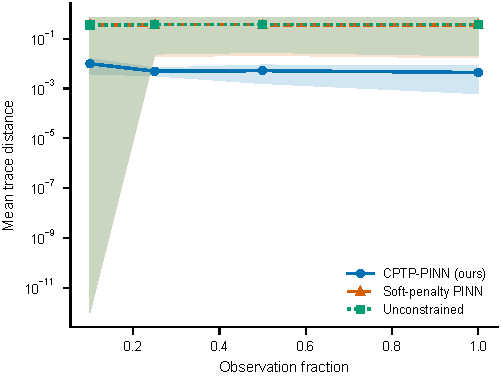
\includegraphics[width=\linewidth]{exp2_sparse_measurements.pdf}\end{minipage}\hfill
    \begin{minipage}[t]{0.31\textwidth}\textbf{b}\\[-0.5ex]
        \centering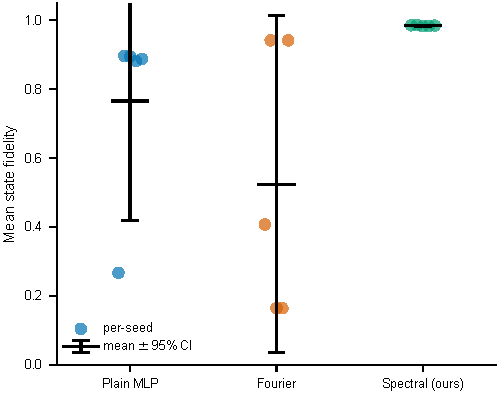
\includegraphics[width=\linewidth]{exp3_qutrit_leakage.pdf}\end{minipage}\hfill
    \begin{minipage}[t]{0.33\textwidth}\textbf{c}\\[-0.5ex]
        \centering
\includegraphics[width=\linewidth]{exp4_gate_fidelity.pdf}\end{minipage}
    \caption{\textbf{Robustness, the spectral-frame cure, and generalization across systems.} \textbf{a}, Sparse-measurement ablation on the single qubit: mean trace distance to the exact trajectory versus retained observation fraction (log scale), for the CPTP-PINN, a soft-penalty PINN and an unconstrained network. \textbf{b}, Fast qutrit reconstruction: per-seed mean state fidelity for the plain MLP, the Fourier-feature density network, and the spectral-frame (interaction-picture) density network. The plain and Fourier baselines are unreliable across seeds, whereas the spectral frame reconstructs the fast dynamics reliably (tight interval near unity)---resolving the principal open problem. \textbf{c}, Two-qubit dissipative gate: state fidelity for the trained $\ket{00}$ trajectory and for three held-out initial states obtained by propagating the learned generator (representative seed). Error bars/bands and points are over five random seeds; see Table~\ref{tab:exp2} and Extended Data Tables~\ref{tab:exp3} and~\ref{tab:exp4}.}
    \label{fig:robustness}
\end{figure}

\subsection{Dense-versus-structured compiler scaling}
\label{sec:experiment_compiler}

The compiler experiment compares dense superoperator evaluation against structured matrix-free residual evaluation on random Lindblad systems: dense mode forms the $d^2\times d^2$ Liouvillian, structured mode evaluates commutator and dissipator terms directly from $H$ and the jump operators. The robust, hardware-independent conclusion is the \emph{memory} separation (Extended Data Table~\ref{tab:exp5}, Figure~\ref{fig:compiler}): consistent with Theorem~\ref{thm:compiler}, dense storage scales as $d^4$, whereas the structured representation stores only $H$, the $m$ jump operators, and $\rho$, i.e.\ $O(md^2)$, so its memory advantage widens with $d$. The two residuals agree to floating-point precision, so structured evaluation is exact, not an approximation. We deliberately do \emph{not} claim a speed advantage: our benchmark's dense path reconstructs the full Liouvillian on every state evaluation (an $O(md^4)$ build paid per state), so the wall-clock gap it reports reflects that implementation artifact rather than an intrinsic per-matvec speedup, and amortizing the Liouvillian build across states would largely remove it. We therefore report timing only as an implementation detail and treat the $O(d^4)$-versus-$O(md^2)$ memory scaling as the genuine, asymptotic separation.

\begin{figure}[t]
    \centering
    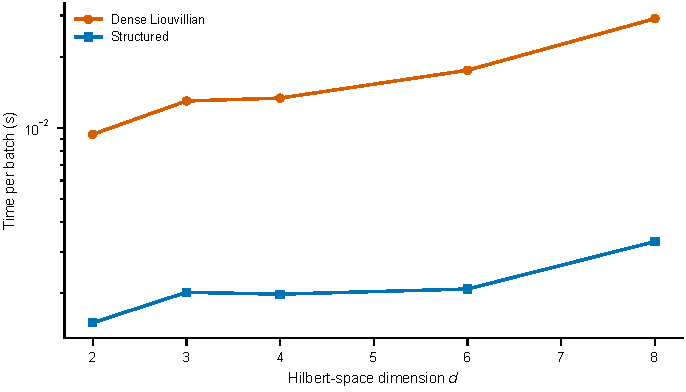
\includegraphics[width=0.55\textwidth]{exp5_compiler_scaling.pdf}
    \caption{\textbf{Matrix-free compiler scaling.} Dense superoperator residual-evaluation time versus structured matrix-free evaluation (median over 50 repeats, log scale). The structured path avoids materializing the $d^2\times d^2$ Liouvillian; its robust advantage is memory ($O(md^2)$ versus $O(d^4)$), not speed---the dense timings shown rebuild the Liouvillian per state and so overstate any wall-clock gap (see text and Extended Data Table~\ref{tab:exp5}).}
    \label{fig:compiler}
\end{figure}

\subsection{Operator-system spectral truncation of the generator}
\label{sec:experiment_truncation}

The final experiment realizes the operator-system spectral truncation of Theorem~\ref{thm:truncation} as a numerical object. A driven, dissipative two-qubit system---large local detunings $\Delta_1=2\pi(5.0)$, $\Delta_2=2\pi(4.8)$, a strong time-dependent exchange coupling $J(t)(XX{+}YY)$ with $J_0=2\pi(0.4)$, and local amplitude damping---is moved into the interaction picture set by the detunings, where the generator $\widetilde\calL_t$ is almost periodic. We extract its Fourier modes $\{\calL_k\}$, keep the band $|k|\le N$, propagate the level-$N$ truncated generator (re-rotating the envelope to the lab frame), and measure the mean state fidelity to the exact trajectory together with the out-of-band weight $\eta_N=\sum_{|k|>N}\norm{\calL_k}$ that certifies the generator-approximation error. Figure~\ref{fig:truncation} and Extended Data Table~\ref{tab:exp6} show a controlled multi-resolution hierarchy: the secular (Davies) generator $N{=}0$ already captures the slow envelope at mean fidelity $\sync{0.76}$; the rotating-wave approximation $N{=}1$ reaches $\sync{0.96}$; and the fidelity converges monotonically to floating-point precision as the band is widened ($\sync{0.99999}$ by $N{=}4$), with $\eta_N$ decreasing in lock-step. The full band reproduces the structured kernel exactly, so the truncation interpolates---with an a~posteriori certificate at every level---between the cheapest time-independent secular model and the exact generator. This is the spectral-truncation construction of noncommutative geometry and $C^*$-algebraic kernel machines~\cite{connes2021spectral,hashimoto2024spectral}, here instantiated for a completely positive dynamical generator.

\begin{figure}[t]
    \centering
    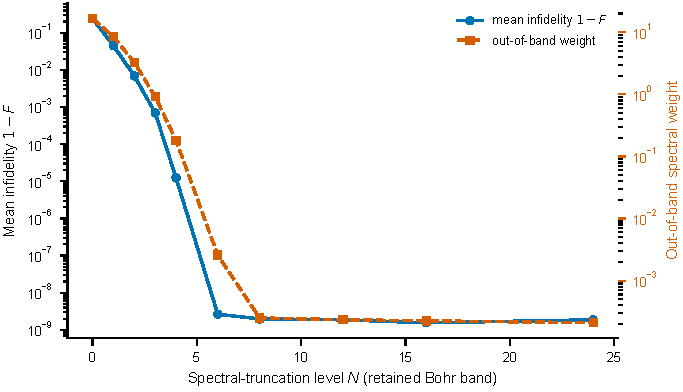
\includegraphics[width=0.6\textwidth]{exp6_spectral_truncation.pdf}
    \caption{\textbf{Operator-system spectral truncation of the open-system generator.} Mean infidelity $1-F$ of the propagated level-$N$ truncated interaction-picture generator (left axis) and the out-of-band spectral weight $\eta_N=\sum_{|k|>N}\norm{\calL_k}$ of Theorem~\ref{thm:truncation} (right axis, log scale) versus the retained Bohr-band level $N$, for a driven dissipative two-qubit system. $N{=}0$ is the secular (Davies) generator, $N{=}1$ the rotating-wave approximation, and the full band recovers the exact generator (and the structured kernel) to floating-point precision. The certificate $\eta_N$ tracks and bounds the infidelity, decreasing monotonically to zero. Deterministic (no seed averaging).}
    \label{fig:truncation}
\end{figure}

% ============================================================
\section{Discussion}
\label{sec:discussion}

The experiments separate what the architectural ingredients---the hard density constraint, the spectral frame, and the matrix-free compiler---each contribute, and where the approach still falls short. We discuss these in turn, then the optimization geometry that governs both.

\paragraph{What the spectral frame buys.}
The hard density constraint guarantees a \emph{physical} trajectory but not an \emph{accurate} one: on fast multi-level dynamics a smooth density network is biased toward low frequencies and cannot resolve the Bohr oscillations, which was the principal failure of the earlier approach. The spectral frame separates the two: the unitary $U(t)=e^{-\ii Ht}$ carries the fast, exactly-known oscillation analytically, and the network learns only the slow envelope through the same hard map. The change is not a new loss or a tuned encoding but a change of \emph{representation}---the eigen-operator decomposition of the dynamics---so it inherits the physicality guarantee (Theorem~\ref{thm:spectral_frame}) while removing spectral bias. Empirically this turns an unreliable reconstruction (mean fidelity $\approx0.5$--$0.8$, intervals as wide as the means) into a reliable one ($\sync{0.985}\pm\sync{0.002}$) and, by making the envelope derivative well conditioned, reduces rate identification to a measurement-noise problem rather than an optimization one. The same eigen-operator decomposition supplies the operator-system spectral truncation: band-limiting the generator to its slow Bohr modes is, mathematically, the spectral truncation by which noncommutative geometry approximates a $C^*$-algebra by finite operator systems~\cite{connes2021spectral,hashimoto2024spectral}, now applied to a completely positive dynamical generator and equipped with a computable error certificate. The secular (Davies) and rotating-wave approximations emerge as its coarsest two levels, and the exact generator as the full band---so a single dial trades cost for fidelity with an a~posteriori guarantee at every setting.

\paragraph{What the hard constraint buys.}
The Cholesky map changes the feasible set. A soft penalty for positivity competes with data fit, residual fit, and optimizer noise; a hard parameterization removes that competition. On the full-data single-qubit problem this is already visible in the \emph{neural} comparison: the CPTP-PINN recovers every parameter far more accurately than the soft-penalty and unconstrained networks and never leaves the physical set, while those baselines do. The only method that beats it there is a classical least-squares fit that already knows the exact model---an honest reference we report rather than omit, and one whose advantage is confined to the dense-data, low-parameter setting. The architectural constraint pays off most clearly in two places the experiments isolate: it guarantees a physical trajectory at every step (zero positivity violations), and it degrades gracefully under sparse measurements (Sec.~\ref{sec:experiment_sparse}), where the soft and unconstrained surrogates leave or fight the positive cone. In larger systems, where the positive cone is a small subset of Hermitian trace-one matrices, this gap is expected to widen.

\paragraph{What the compiler buys.}
The compiler determines whether the residual can be evaluated without forming an object whose size scales as $d^4$. In a multi-qubit Hilbert space $d=2^n$, so dense Liouvillian storage scales as $16^n$; structured kernels still face exponential Hilbert-space growth but avoid an unnecessary square of the density-vector dimension. This is the difference between a prototype that only runs on toy models and a path that can exploit locality, batching, sparsity, tensor products, and GPU memory hierarchy. The most direct accelerator path lowers each Hamiltonian and dissipator term to batched matrix multiplications, fuses anticommutator terms, and keeps density matrices resident on GPU; circuit- or pulse-level noise hypotheses can be compiled into Hamiltonian and jump-operator terms via existing stacks~\cite{qiskit2024,qutip2024}, and resource-estimation tools may interact with learned models~\cite{beverland2022assessing,rall2023quantum}.

\paragraph{Optimization geometry and failure modes.}
The Cholesky map is nonlinear and redundant; near rank-deficient states, small changes in the factor can produce small eigenvalues and ill-conditioning. This is a reason for careful initialization, diagonal floors, learning-rate schedules, and low-rank-plus-isotropic variants, not a reason to abandon the representation. The framework has three distinct diagnostics that should not be conflated (Methods, Sec.~\ref{sec:gauge_failure_modes}): state physicality (guaranteed), residual size, and held-out prediction error. A model can be physical at every time and still solve the wrong dynamics; only the residual and held-out validation certify the model, and only an identifiability analysis (Theorem~\ref{thm:identifiability}) certifies the parameters.

\subsection{Limitations}
\label{sec:limitations}

\begin{enumerate}[leftmargin=1.5em]
    \item \textbf{Rate sloppiness under measurement noise.} The spectral frame resolves the fast-reconstruction problem (Sec.~\ref{sec:experiment_qutrit}), so what remains is a measurement-noise question: with the trajectory reliably reconstructed, the dominant decay rates are recovered, but a weakly excited rate (the qutrit dephasing $\gamma_\phi$) is a sloppy direction at $2\%$ noise, exactly as the local identifiability bound (Theorem~\ref{thm:identifiability}) predicts---the readout is exact on the noiseless envelope. Richer measurement designs (active experiment design that maximizes the smallest singular value of the sensitivity Gramian) and derivative denoising are the natural next steps.
    \item \textbf{Known frame Hamiltonian.} The spectral frame and the operator-system truncation use the eigenbasis of a \emph{known} coherent part $H$. When $H$ itself is unknown or strongly time-dependent, the frame must be co-learned or chosen adaptively; a partial frame (the dominant static part) still removes the fast oscillations, as in the two-qubit experiments.
    \item \textbf{No hardware data.} The experiments are synthetic CPU simulations; they test the implementation and theory but do not demonstrate performance on a quantum device.
    \item \textbf{Markovian assumption.} The framework assumes GKSL dynamics. Non-Markovian systems require extended state spaces, memory kernels, or process tensors.
    \item \textbf{Identifiability is measurement-dependent.} The theorems cannot overcome uninformative observables: if the sensitivity Gramian is rank deficient, no optimizer can recover all parameters.
    \item \textbf{Scope of the empirical claims.} The study is a small proof of concept (five seeds per experiment); it is not benchmarked against every modern system-identification method, and it does not claim state of the art.
\end{enumerate}

\paragraph{Conclusion.}
Spectral-CPTP-PINNs combine a physical state parameterization, a spectral-frame eigen-operator representation, an operator-system spectral truncation of the generator, generator learning that preserves the GKSL form, and matrix-free residual compilation. The conceptual point is twofold: physicality should be an architectural invariant rather than a penalty applied after the fact, and the fast coherent structure of open-system dynamics should be carried by an analytic change of frame rather than learned, so that the network represents only what is genuinely unknown. The mathematics shows that these choices do not destroy universal approximation, that the learned generator remains CPTP, that the spectral frame is exactly physical and exactly equivalent to the lab dynamics, that residuals and the spectral-truncation tail provide a~posteriori certificates, and that structured compilation avoids dense Liouvillian storage. The spectral truncation moreover gives a controlled bridge---the secular and rotating-wave approximations as its coarsest levels---between the cheapest time-independent generator and the exact one. The experiments are deliberately modest but authentic and statistically reported. Future work should extend to larger multi-qubit systems, co-learned or adaptive frames, hardware-calibration datasets, non-Markovian embeddings, and GPU-native kernels; the most promising engineering direction is a compiler that takes a high-level noise model and emits fused, batched, spectrally truncated, differentiable kernels for accelerator execution.

% ============================================================
\section{Methods}
\label{sec:methods}

\subsection{Background: GKSL dynamics and dense Liouvillian}
\label{sec:gksl}
Let $\rho(t)\in\calD(\hilb)$. A time-independent Markovian master equation has the form
\begin{equation}
    \frac{\dd\rho}{\dd t}=\calL_\Theta[\rho]=-\ii[H_\Theta,\rho]+\sum_{k=1}^{m}\gamma_k\!\left(L_k\rho L_k^\dagger-\tfrac12\{L_k^\dagger L_k,\rho\}\right),
    \label{eq:gksl_rates}
\end{equation}
with $H_\Theta=H_\Theta^\dagger$, $\gamma_k\ge0$; the GKSL theorem characterizes generators of quantum dynamical semigroups in finite dimensions~\cite{lindblad1976generators,gorini1976completely,breuer2002theory,wiseman2009quantum}. Using the column-major identity $\operatorname{vec}(A\rho B)=(B^T\otimes A)\operatorname{vec}(\rho)$, the dense Liouvillian is
\begin{equation}
    \mathbb{L}_\Theta=-\ii(I\otimes H_\Theta-H_\Theta^T\otimes I)+\sum_k\gamma_k\!\left(L_k^*\otimes L_k-\tfrac12 I\otimes L_k^\dagger L_k-\tfrac12 (L_k^\dagger L_k)^T\otimes I\right),
    \label{eq:dense_liouvillian}
\end{equation}
which stores $d^4$ complex scalars, whereas direct evaluation of~\eqref{eq:gksl_rates} stores $H$ and the $L_k$, i.e.\ $O(md^2)$.

\subsection{Generator parameterization (details)}
\label{sec:generator_parameterization}
For known jump operators with unknown rates,
\begin{equation}
    \gamma_k(\xi_k)=\softplus(\xi_k)+\gamma_{\min},\qquad\gamma_{\min}\ge0;
    \label{eq:softplus_rates}
\end{equation}
for a full Kossakowski matrix in a fixed basis $\{F_a\}_{a=1}^{q}$, $C_\eta=B_\eta B_\eta^\dagger\succeq0$ and
\begin{equation}
    \calL_\Theta[\rho]=-\ii[H_\Theta,\rho]+\sum_{a,b=1}^{q}(C_\eta)_{ab}\!\left(F_a\rho F_b^\dagger-\tfrac12\{F_b^\dagger F_a,\rho\}\right),
    \label{eq:kossakowski_generator}
\end{equation}
with $H_\theta(t)=\sum_\ell\theta_\ell(t)G_\ell$, $G_\ell=G_\ell^\dagger$.

\subsection{Observation model and loss (details)}
\label{sec:loss}
With observables $\{O_j\}_{j=1}^{p}$, measurements $y_{ij}$ at time $t_i$, and masks $m_{ij}\in\{0,1\}$,
\begin{equation}
    \calJ_{\rm data}(\phi)=\frac{1}{\sum_{i,j}m_{ij}}\sum_{i,j}m_{ij}\!\left(\Tr[O_j\rhophi(t_i)]-y_{ij}\right)^2,\quad
    \calJ_0(\phi)=\norm{\rhophi(0)-\rho_0}_F^2,
    \label{eq:data_ic_loss}
\end{equation}
and $\calJ_{\rm phys}$ as in~\eqref{eq:pinn_general_loss}. The derivative $\dot\rhophi$ is obtained by automatic differentiation; the centered finite-difference surrogate $\dot\rhophi(t)\approx[\rhophi(t+h)-\rhophi(t-h)]/2h$ is an alternative. The soft-penalty baseline adds $\lambda_{\rm pos}\sum_i\mathrm{ReLU}(-\lambda_i(\rho))$ to the loss. We use Adam~\cite{kingma2015adam}; L-BFGS is a natural second stage~\cite{liu1989limited}.

\subsection{Spectral-frame parameterization and interaction-picture residual}
\label{sec:spectral_methods}
Let $H=\sum_a E_a\proj{a}$ be the (known) frame Hamiltonian in its eigenbasis and $U(t)=e^{-\ii H t}$. The spectral-frame density network outputs an envelope $\widetilde\rho_\phi(t)\in\calD(\hilb)$ in the eigenbasis through the same Cholesky map~\eqref{eq:intro_cholesky}, and the lab state is the analytic rotation
\begin{equation}
    \rhophi(t)=U(t)\,\widetilde\rho_\phi(t)\,U(t)^\dagger,\qquad
    (\widetilde\rho_\phi)_{ab}\mapsto e^{-\ii\omega_{ab}t}(\widetilde\rho_\phi)_{ab}\ \text{(Hadamard)},
    \label{eq:spectral_rotation}
\end{equation}
with Bohr frequencies $\omega_{ab}=E_a-E_b$; for diagonal $H$ the rotation is the entrywise phase $e^{-\ii\omega_{ab}t}$. Because $U(t)$ is unitary, $\rhophi(t)\in\calD(\hilb)$ by Theorem~\ref{thm:spectral_frame}. The data and initial-condition terms~\eqref{eq:data_ic_loss} use $\rhophi$; the physics residual is evaluated in the interaction picture,
\begin{equation}
    \calJ_{\rm phys}^{\rm spec}=\tfrac{1}{N_c}\sum_\ell\norm{\dot{\widetilde\rho}_\phi(\tau_\ell)-\widetilde\calL_{\Theta,\tau_\ell}[\widetilde\rho_\phi(\tau_\ell)]}_F^2,\qquad
    \widetilde L_k(t)=e^{\ii\omega_{ab}t}(L_k)_{ab},
    \label{eq:spectral_residual}
\end{equation}
where $\dot{\widetilde\rho}_\phi$ is the autodiff derivative of the \emph{slow} envelope and $\widetilde\calL_{\Theta,t}$ is the GKSL generator of Theorem~\ref{thm:spectral_frame}; for single-transition jump operators $\widetilde\calL_{\Theta,t}$ is time-independent. Because $\widetilde\rho_\phi$ is slowly varying, $\dot{\widetilde\rho}_\phi$ is far better conditioned under measurement noise than the lab-frame derivative, which is what makes the dissipative rates recoverable. We therefore add a \emph{two-stage rate readout}: the interaction-picture generator is linear in the rates, $\dot{\widetilde\rho}=\sum_k\gamma_k\calD_k[\widetilde\rho]$ with $\calD_k[\rho]=L_k\rho L_k^\dagger-\tfrac12\{L_k^\dagger L_k,\rho\}$, so after fitting the envelope we solve the small nonnegative least-squares problem $\min_{\gamma\ge0}\sum_i\norm{\dot{\widetilde\rho}_\phi(t_i)-\sum_k\gamma_k\calD_k[\widetilde\rho_\phi(t_i)]}_F^2$---the operational form of the identifiability bound (Theorem~\ref{thm:identifiability}).

\subsection{Operator-system spectral truncation of the generator}
\label{sec:truncation_methods}
The interaction-picture generator $\widetilde\calL_t$ is almost periodic; on $[0,T]$ it admits the Fourier series $\widetilde\calL_t=\sum_k e^{\ii k\omega_0 t}\calL_k$, $\omega_0=2\pi/T$, whose modes $\calL_k=\tfrac1T\int_0^T e^{-\ii k\omega_0 t}\widetilde\calL_t\,\dd t$ we obtain by a temporal FFT of the dense superoperator on a uniform grid. The \emph{level-$N$ spectral truncation} keeps the band $|k|\le N$, $\widetilde\calL_t^{(N)}=\sum_{|k|\le N}e^{\ii k\omega_0 t}\calL_k$---a projection onto the finite operator system spanned by the slow eigen-operators, in the sense of Connes--van Suijlekom~\cite{connes2021spectral,vansuijlekom2021gromov}. Retaining $\calL_0$ and conjugate-symmetric pairs $\calL_{\pm k}$ keeps the truncated generator Hermiticity- and trace-preserving; $N=0$ is the time-independent secular (Davies) generator~\cite{davies1974markovian} and $N=1$ the rotating-wave approximation. The out-of-band weight $\eta_N=\sum_{|k|>N}\norm{\calL_k}$ is the a~posteriori certificate of Theorem~\ref{thm:truncation}; the full band reproduces the structured kernel of~\eqref{eq:gksl_rates} exactly.

\subsection{Open-system IR, dispatch, and algorithms}
\label{sec:ir}
The compiler receives an IR $\mathsf{IR}=(d,\{G_\ell\},\{F_a\},\Theta,\{O_j\},\mathsf{batch},\mathsf{mode})$. Dense mode constructs~\eqref{eq:dense_liouvillian}; structured mode evaluates~\eqref{eq:gksl_rates} directly and is the default when $d$ is large, $m$ is small, or the computation is batched. A practical dispatch rule is
\begin{equation}
    \mathsf{mode}=\begin{cases}\mathsf{dense},& d\le d_{\rm dense}\text{ and }N_{\rm batch}\text{ small},\\ \mathsf{structured},& md^2\ll d^4\text{ or }N_{\rm batch}\text{ large},\\ \mathsf{tensor},& H,L_k\text{ are sums of tensor-local terms.}\end{cases}
\end{equation}
Thresholds should be empirical because BLAS libraries, GPU memory, and batch sizes move the crossover.

\begin{algorithm}[h]
\caption{Residual-kernel dispatch from an open-system IR}
\label{alg:dispatch}
\begin{algorithmic}[1]
\REQUIRE IR with dimension $d$, jump count $m$, sparsity/tensor metadata, batch size $N_b$, device.
\IF{tensor-local metadata available and tensor backend enabled}
    \STATE return tensor-local residual kernel.
\ELSIF{$d^4$ storage fits device memory and $d\le d_{\rm dense}$}
    \STATE materialize dense Liouvillian; return dense matvec kernel.
\ELSIF{operators are sparse}
    \STATE return sparse structured kernel.
\ELSE
    \STATE return dense-matrix structured kernel (commutator and dissipators term by term).
\ENDIF
\STATE Attach gradient rule: automatic differentiation, custom adjoint, or finite-difference fallback.
\end{algorithmic}
\end{algorithm}

\begin{algorithm}[h]
\caption{CPTP-Compiler-PINN training}
\label{alg:cptp_compiler_pinn}
\begin{algorithmic}[1]
\REQUIRE Observations $\{(t_i,O_j,y_{ij},m_{ij})\}$, initial state $\rho_0$, Hamiltonian basis $\{G_\ell\}$, jump/Kossakowski basis, collocation grid $\{\tau_\ell\}$.
\ENSURE Density surrogate $\rhophi(t)$ and generator parameters $\Theta$.
\STATE Initialize $\phi$ and unconstrained generator parameters $\xi$; compile the IR to a residual evaluator.
\FOR{step $s=1,\ldots,S$}
    \STATE Form $A_\phi(t)$ by~\eqref{eq:A_definition} and $\rhophi(t)$ by~\eqref{eq:intro_cholesky}; map rates by~\eqref{eq:softplus_rates} or $C=BB^\dagger$.
    \STATE Evaluate predictions $\Tr[O_j\rhophi(t_i)]$, derivative $\dot\rhophi(\tau_\ell)$, and $\calL_\Theta[\rhophi(\tau_\ell)]$.
    \STATE Compute $\calJ=\lambda_{\rm data}\calJ_{\rm data}+\lambda_{\rm phys}\calJ_{\rm phys}+\lambda_0\calJ_0$; update $(\phi,\xi)$ with Adam.
\ENDFOR
\STATE Return $(\phi,\Theta)$ and the residual certificate of Theorem~\ref{thm:certificate}.
\end{algorithmic}
\end{algorithm}

\begin{algorithm}[h]
\caption{Spectral-frame training and rate readout}
\label{alg:spectral}
\begin{algorithmic}[1]
\REQUIRE Observations $\{(t_i,O_j,y_{ij})\}$, initial state $\rho_0$, frame Hamiltonian $H$, jump operators $\{L_k\}$, collocation grid $\{\tau_\ell\}$.
\ENSURE Lab trajectory $\rhophi(t)$, fitted rates $\gamma$.
\STATE Diagonalize $H=\sum_aE_a\proj{a}$; precompute the Bohr phases $e^{\ii\omega_{ab}t}$ and the eigenbasis jump operators $\widetilde L_k=U^\dagger L_kU$.
\FOR{step $s=1,\ldots,S$}
    \STATE Form the envelope $\widetilde\rho_\phi(t)$ by~\eqref{eq:A_definition}--\eqref{eq:intro_cholesky} and the lab state $\rhophi(t)=U(t)\widetilde\rho_\phi(t)U(t)^\dagger$ by~\eqref{eq:spectral_rotation}.
    \STATE Evaluate $\Tr[O_j\rhophi(t_i)]$ for the data term and the interaction-picture residual~\eqref{eq:spectral_residual} for $\calJ_{\rm phys}^{\rm spec}$; update $(\phi,\xi)$ with Adam.
\ENDFOR
\STATE \textbf{Rate readout:} with the trained envelope, solve $\min_{\gamma\ge0}\sum_i\norm{\widetilde\rho_\phi(t_i)-e^{t_i\sum_k\gamma_k\calD_k}\widetilde\rho_\phi(0)}_F^2$ (integral form) or the derivative least squares of Sec.~\ref{sec:spectral_methods}.
\STATE Return $\rhophi$ and $\gamma$.
\end{algorithmic}
\end{algorithm}

\begin{algorithm}[h]
\caption{Operator-system spectral truncation of the generator}
\label{alg:truncation}
\begin{algorithmic}[1]
\REQUIRE Frame $H$, residual coherent term $H_c(t)$, jump operators $\{L_k(t)\}$, window $T$, level $N$.
\ENSURE Level-$N$ truncated generator and certificate $\eta_N$.
\STATE Sample the interaction-picture Liouvillian $\widetilde{\mathbb L}(t_g)$ on a uniform grid; take a temporal FFT to obtain Fourier modes $\{\calL_k\}$.
\STATE Keep the band $|k|\le N$ (the $k{=}0$ mode and conjugate-symmetric pairs); set $\widetilde{\mathbb L}^{(N)}(t)=\sum_{|k|\le N}e^{\ii k\omega_0 t}\calL_k$.
\STATE Compute the certificate $\eta_N=\sum_{|k|>N}\norm{\calL_k}$ (Theorem~\ref{thm:truncation}); propagate $\widetilde{\mathbb L}^{(N)}$ and rotate the envelope back to the lab frame as needed.
\end{algorithmic}
\end{algorithm}

\subsection{Proofs}
\label{sec:appendix_proofs}

\begin{proof}[Proof of Theorem~\ref{thm:physicality}]
Fix $t\in[0,T]$ and write $A=A(t)$, $M=AA^\dagger$, $Z=\Tr M$, so that $\rho_A(t)=M/Z$. We verify the three defining properties of $\calD(\hilb)$ in turn, then differentiability.

\emph{(i) Hermiticity.} Taking the conjugate transpose and using $(XY)^\dagger=Y^\dagger X^\dagger$ and $(A^\dagger)^\dagger=A$ gives $M^\dagger=(AA^\dagger)^\dagger=(A^\dagger)^\dagger A^\dagger=AA^\dagger=M$, so $M$ is Hermitian. Since $Z=\Tr M$ is real (the trace of a Hermitian matrix is the sum of its real diagonal entries), $\rho_A=M/Z$ is Hermitian.

\emph{(ii) Positive semidefiniteness.} For any $v\in\C^d$,
\[
v^\dagger M v = v^\dagger A A^\dagger v = (A^\dagger v)^\dagger (A^\dagger v)=\norm{A^\dagger v}_2^2\ge 0,
\]
so $M\succeq0$. We now show $Z>0$. Because $A\ne0$ there is an entry $A_{pq}\ne0$, hence $Z=\Tr(AA^\dagger)=\sum_{i,j}\abs{A_{ij}}^2=\norm{A}_F^2\ge\abs{A_{pq}}^2>0$. Dividing a PSD matrix by a strictly positive scalar preserves positive semidefiniteness, so $\rho_A=M/Z\succeq0$.

\emph{(iii) Unit trace.} By linearity of the trace and $Z=\Tr M$, $\Tr\rho_A=\Tr(M/Z)=(\Tr M)/Z=Z/Z=1$.

Properties (i)--(iii) are exactly the conditions defining $\calD(\hilb)$, so $\rho_A(t)\in\calD(\hilb)$.

\emph{Differentiability and tracelessness of the derivative.} Suppose $A$ is differentiable on $[0,T]$. Then $M(t)=A(t)A(t)^\dagger$ is differentiable with $\dot M=\dot A\,A^\dagger+A\,\dot A^\dagger$ by the product rule, and $Z(t)=\Tr M(t)$ is differentiable with $\dot Z=\Tr\dot M$. Since $Z(t)>0$ for all $t$ by (ii), the quotient $\rho_A=M/Z$ is differentiable on $[0,T]$ with
\[
\dot\rho_A=\frac{\dot M}{Z}-\frac{M\,\dot Z}{Z^2}.
\]
Each term on the right is Hermitian ($\dot M$ is Hermitian because $(\dot A A^\dagger+A\dot A^\dagger)^\dagger=\dot A A^\dagger+A\dot A^\dagger$, and $Z,\dot Z\in\R$), so $\dot\rho_A$ is Hermitian. Finally, differentiating the identity $\Tr\rho_A(t)\equiv1$ from (iii) and using linearity of the trace gives $\Tr\dot\rho_A(t)=\tfrac{\dd}{\dd t}\Tr\rho_A(t)=0$. This holds at every $t$, every training iteration, and every evaluation point, which is exactly the zero positivity-violation rate measured for the Cholesky model in Experiment~1 (Table~\ref{tab:exp1}).
\end{proof}

\begin{proof}[Proof of Theorem~\ref{thm:universal}]
The proof has three steps: (1) regularize the target trajectory so it is uniformly positive definite; (2) extract a continuous Cholesky factor; (3) approximate that factor by a network and push the approximation through the (locally Lipschitz) density map.

\emph{Step 1: regularization.} Fix $\eta\in(0,1)$ and define $\rho_\eta(t)=(1-\eta)\rho(t)+\eta\sigma$. As a convex combination of the state $\rho(t)\succeq0$ and $\sigma\succeq0$ with weights summing to one, $\rho_\eta(t)\in\calD(\hilb)$. Moreover for any unit vector $v$, $v^\dagger\rho_\eta(t)v\ge\eta\, v^\dagger\sigma v\ge\eta\,\lambda_{\min}(\sigma)=:c>0$ because $\sigma$ is full rank; hence $\rho_\eta(t)\succeq cI$ uniformly in $t$, i.e.\ $\rho_\eta$ is uniformly positive definite. Its deviation from the target is bounded by
\[
\sup_t\norm{\rho_\eta(t)-\rho(t)}_F=\sup_t\norm{\eta(\sigma-\rho(t))}_F=\eta\sup_t\norm{\sigma-\rho(t)}_F=:\eta\,K,
\]
where $K<\infty$ because $\rho$ is continuous on the compact interval $[0,T]$ and $\calD(\hilb)$ is bounded. Choose $\eta=\min\{1/2,\ \eps/(2K+1)\}$, so that $\sup_t\norm{\rho_\eta-\rho}_F<\eps/2$.

\emph{Step 2: continuous Cholesky factor.} For each $t$, $\rho_\eta(t)$ is Hermitian positive definite, so it has a unique Cholesky factorization $\rho_\eta(t)=C_\eta(t)C_\eta(t)^\dagger$ with $C_\eta(t)$ lower triangular and strictly positive real diagonal. The Cholesky factor of a Hermitian positive-definite matrix is a smooth (in particular continuous) function of the matrix entries on the open cone of positive-definite matrices, because each entry of $C_\eta$ is obtained from entries of $\rho_\eta$ by the recursive Cholesky formulas, which involve only additions, multiplications, divisions by the strictly positive computed diagonal entries, and square roots of strictly positive computed quantities---all continuous operations on that domain. Since $t\mapsto\rho_\eta(t)$ is continuous and stays in this cone, $t\mapsto C_\eta(t)$ is continuous on $[0,T]$. Collecting the real and imaginary parts of the (at most $d^2$) free lower-triangular entries gives a continuous map $g:[0,T]\to\R^{d^2}$.

\emph{Step 3: network approximation and Lipschitz transfer.} By the universal approximation theorem for feedforward networks with a nonpolynomial activation~\cite{cybenko1989approximation,hornik1991approximation}, for every $\eps'>0$ there is a finite network $\widehat g:[0,T]\to\R^{d^2}$ with $\sup_t\norm{\widehat g(t)-g(t)}_2<\eps'$. Reassembling $\widehat g(t)$ into a lower-triangular complex matrix $A_\phi(t)$ (the same way $g$ was assembled from $C_\eta$) yields a network with $\sup_t\norm{A_\phi(t)-C_\eta(t)}_F<\eps'$. Now consider the density map $\Psi(A)=AA^\dagger/\Tr(AA^\dagger)$. On the compact set $\mathcal{K}=\{A:\norm{A-C_\eta(t)}_F\le1\text{ for some }t\}$, the trace $\Tr(AA^\dagger)=\norm{A}_F^2$ is bounded below by a constant $\beta>0$ (because $\inf_t\norm{C_\eta(t)}_F>0$ by uniform positive definiteness and $\eps'\le1$), and both the numerator $AA^\dagger$ and the denominator are polynomial in the entries of $A$ with the denominator bounded away from zero; hence $\Psi$ is continuously differentiable on $\mathcal{K}$, so by the mean value inequality it is Lipschitz there with some constant $L<\infty$. Therefore, choosing $\eps'=\min\{1,\ \eps/(2L)\}$,
\[
\sup_t\norm{\Psi(A_\phi(t))-\Psi(C_\eta(t))}_F\le L\sup_t\norm{A_\phi(t)-C_\eta(t)}_F< L\,\eps'\le\eps/2.
\]
But $\Psi(C_\eta(t))=C_\eta C_\eta^\dagger/\Tr(C_\eta C_\eta^\dagger)=\rho_\eta(t)/\Tr\rho_\eta(t)=\rho_\eta(t)$ since $\Tr\rho_\eta(t)=1$. Writing $\rho_\phi(t)=\Psi(A_\phi(t))$ and combining with Step 1 via the triangle inequality,
\[
\sup_t\norm{\rho_\phi(t)-\rho(t)}_F\le\sup_t\norm{\rho_\phi(t)-\rho_\eta(t)}_F+\sup_t\norm{\rho_\eta(t)-\rho(t)}_F<\tfrac{\eps}{2}+\tfrac{\eps}{2}=\eps,
\]
and $A_\phi$ has nonzero output everywhere because $\norm{A_\phi(t)}_F\ge\norm{C_\eta(t)}_F-\eps'>0$. This is an \emph{approximation} (existence) guarantee on the hypothesis class; it does not assert that gradient-based optimization will find such a network, and indeed the training objective remains nonconvex---a fragility made explicit by the seed variance of the qutrit reconstruction (Experiment~3, Extended Data Table~\ref{tab:exp3}).
\end{proof}

\begin{proof}[Proof of Theorem~\ref{thm:cptp_generator}]
We treat the two parameterizations separately and in both cases reduce the learned generator to the canonical GKSL form whose exponential is CPTP by the Gorini--Kossakowski--Sudarshan--Lindblad theorem~\cite{lindblad1976generators,gorini1976completely,breuer2002theory}, which states that a linear map $\calL$ on $d\times d$ matrices generates a completely positive trace-preserving semigroup $\{e^{t\calL}\}_{t\ge0}$ if and only if it can be written as
\begin{equation}
\calL[\rho]=-\ii[H,\rho]+\sum_{r}\Big(V_r\rho V_r^\dagger-\tfrac12\{V_r^\dagger V_r,\rho\}\Big),\qquad H=H^\dagger.
\label{eq:canonical_gksl}
\end{equation}

\emph{Rate parameterization.} The Hamiltonian $H_\theta=\sum_\ell\theta_\ell G_\ell$ with $G_\ell=G_\ell^\dagger$ and $\theta_\ell\in\R$ is Hermitian because $H_\theta^\dagger=\sum_\ell\theta_\ell G_\ell^\dagger=\sum_\ell\theta_\ell G_\ell=H_\theta$. For each rate, $\softplus(x)=\ln(1+e^x)>0$ for all $x\in\R$ (the argument $1+e^x>1$, and $\ln$ is positive on $(1,\infty)$); adding $\gamma_{\min}\ge0$ keeps $\gamma_k(\xi_k)=\softplus(\xi_k)+\gamma_{\min}>0$. Setting $V_k=\sqrt{\gamma_k}\,L_k$ absorbs each nonnegative rate into its jump operator, and $V_k\rho V_k^\dagger=\gamma_k L_k\rho L_k^\dagger$, $V_k^\dagger V_k=\gamma_k L_k^\dagger L_k$, so~\eqref{eq:gksl_rates} is exactly~\eqref{eq:canonical_gksl} with $V_k=\sqrt{\gamma_k}L_k$. Hence $e^{t\calL_\Theta}$ is CPTP for all $t\ge0$.

\emph{Kossakowski parameterization.} Here $\calL_\Theta[\rho]=-\ii[H_\Theta,\rho]+\sum_{a,b=1}^q(C)_{ab}\big(F_a\rho F_b^\dagger-\tfrac12\{F_b^\dagger F_a,\rho\}\big)$ with $C=BB^\dagger$. The matrix $C$ is Hermitian, since $C^\dagger=(BB^\dagger)^\dagger=BB^\dagger=C$, and PSD, since $u^\dagger C u=u^\dagger BB^\dagger u=\norm{B^\dagger u}_2^2\ge0$ for all $u\in\C^q$. By the spectral theorem there is a unitary $U$ and nonnegative eigenvalues $\Lambda_r\ge0$ with $C=U\Lambda U^\dagger$, i.e.\ $C_{ab}=\sum_r U_{ar}\Lambda_r\overline{U_{br}}$. Define the rotated operators $\widetilde L_r=\sqrt{\Lambda_r}\sum_a U_{ar}F_a$. Substituting $C_{ab}=\sum_r U_{ar}\Lambda_r\overline{U_{br}}$ and exchanging the finite sums,
\[
\sum_{a,b}C_{ab}F_a\rho F_b^\dagger=\sum_r\Lambda_r\Big(\sum_a U_{ar}F_a\Big)\rho\Big(\sum_b U_{br}F_b\Big)^\dagger=\sum_r\widetilde L_r\rho\widetilde L_r^\dagger,
\]
where the last equality uses $\big(\sum_b U_{br}F_b\big)^\dagger=\sum_b\overline{U_{br}}F_b^\dagger$ and $\Lambda_r=(\sqrt{\Lambda_r})^2$; the identical computation applied to the anticommutator term gives $\sum_{a,b}C_{ab}F_b^\dagger F_a=\sum_r\widetilde L_r^\dagger\widetilde L_r$. Therefore $\calL_\Theta$ equals~\eqref{eq:canonical_gksl} with $V_r=\widetilde L_r$ and the same Hermitian $H_\Theta$, so it too generates a CPTP semigroup. Trace preservation holds in both cases because each term of~\eqref{eq:canonical_gksl} is traceless ($\Tr[H,\rho]=0$ by cyclicity, and $\Tr(V_r\rho V_r^\dagger)=\Tr(V_r^\dagger V_r\rho)=\tfrac12\Tr\{V_r^\dagger V_r,\rho\}$). This architectural guarantee is what makes the learned two-qubit generator a legal Lindbladian that can be propagated to held-out initial states (Experiment~4, Extended Data Table~\ref{tab:exp4}).
\end{proof}

\begin{proof}[Proof of Theorem~\ref{thm:certificate}]
Let $\Phi_t=e^{t\calL}$ be the CPTP semigroup generated by $\calL$ and set the error path $e(t)=\rhohat(t)-\rho(t)$.

\emph{Step 1: an inhomogeneous linear ODE for the error.} Both $\rhohat$ and $\rho$ are differentiable. Using $\dot\rho=\calL[\rho]$ and $\dot\rhohat=\calL[\rhohat]+r$ (the definition of the residual $r=\dot\rhohat-\calL[\rhohat]$),
\[
\dot e(t)=\dot\rhohat(t)-\dot\rho(t)=\big(\calL[\rhohat]+r\big)-\calL[\rho]=\calL[e(t)]+r(t),
\]
by linearity of $\calL$. This is a linear inhomogeneous ODE with constant generator $\calL$ and forcing $r$.

\emph{Step 2: variation of constants.} The unique solution of $\dot e=\calL[e]+r$ with initial value $e(0)$ is, by Duhamel's formula (verified by differentiating the right-hand side and using $\tfrac{\dd}{\dd t}\Phi_t=\calL\Phi_t=\Phi_t\calL$),
\[
e(t)=\Phi_t[e(0)]+\int_0^t\Phi_{t-s}[r(s)]\,\dd s.
\]

\emph{Step 3: $r(s)$ is Hermitian and traceless.} By hypothesis $\rhohat$ is a Hermitian, trace-one path, so $\dot\rhohat$ is Hermitian (the derivative of a Hermitian-valued path is Hermitian) and $\Tr\dot\rhohat=\tfrac{\dd}{\dd t}\Tr\rhohat=\tfrac{\dd}{\dd t}1=0$. The generator $\calL$ maps Hermitian inputs to Hermitian outputs and is trace annihilating ($\Tr\calL[X]=0$ for all $X$, since each GKSL term is traceless). Hence $r=\dot\rhohat-\calL[\rhohat]$ is Hermitian with $\Tr r(s)=0$.

\emph{Step 4: a CPTP map is a trace-norm contraction on Hermitian traceless matrices.} Let $X$ be Hermitian with $\Tr X=0$. By the spectral theorem write the Jordan (positive/negative) decomposition $X=X_+-X_-$ with $X_\pm\succeq0$ supported on orthogonal eigenspaces; then $\norm{X}_1=\Tr X_++\Tr X_-$ and $\Tr X=\Tr X_+-\Tr X_-=0$ forces $\Tr X_+=\Tr X_-=:a$, so $\norm{X}_1=2a$. If $a=0$ then $X=0$ and the claim is trivial; otherwise set $\rho_\pm=X_\pm/a$, which are density matrices, and $X=a(\rho_+-\rho_-)$. Because $\Phi$ is CPTP it maps density matrices to density matrices, and the trace distance $\tfrac12\norm{\cdot}_1$ is contractive under any CPTP map (the Holevo--Helstrom monotonicity of trace distance). Therefore, using linearity and homogeneity of $\Phi$ and the norm,
\[
\tfrac12\norm{\Phi[X]}_1=\tfrac12\norm{a\big(\Phi[\rho_+]-\Phi[\rho_-]\big)}_1=a\cdot\tfrac12\norm{\Phi[\rho_+]-\Phi[\rho_-]}_1\le a\cdot\tfrac12\norm{\rho_+-\rho_-}_1=a=\tfrac12\norm{X}_1.
\]
Thus $\norm{\Phi[X]}_1\le\norm{X}_1$ for every Hermitian traceless $X$, and in particular for each $\Phi_{t-s}$ applied to the Hermitian traceless $e(0)$ and $r(s)$.

\emph{Step 5: assembling the bound.} Take the trace norm of the variation-of-constants formula, apply the triangle inequality (for the integral, $\norm{\int_0^t g\,\dd s}_1\le\int_0^t\norm{g}_1\,\dd s$), and then the contraction of Step 4 to each $\Phi$:
\[
\tfrac12\norm{e(t)}_1\le\tfrac12\norm{\Phi_t[e(0)]}_1+\tfrac12\int_0^t\norm{\Phi_{t-s}[r(s)]}_1\,\dd s\le\tfrac12\norm{e(0)}_1+\tfrac12\int_0^t\norm{r(s)}_1\,\dd s,
\]
which is exactly~\eqref{eq:certificate}. The right-hand side is computable from the learned path alone (it never references the unknown $\rho$), so a small training residual is an a~posteriori guarantee; the bound is verified empirically on physical perturbations of the exact qubit trajectory in Extended Data Table~\ref{tab:residual_certificate}, where the certificate stays a small constant factor above the true error.
\end{proof}

\begin{proof}[Proof of Theorem~\ref{thm:identifiability}]
Write $\Delta=\Thetahat-\Theta_*\in\R^q$ and define $\gamma(\alpha)=\Theta_*+\alpha\Delta$ for $\alpha\in[0,1]$, the straight segment from $\Theta_*$ to $\Thetahat$. Since $f$ is continuously differentiable (the observation map is a smooth function of the generator parameters, the solution of a smooth ODE depending smoothly on parameters being smooth), the fundamental theorem of calculus applied to $\alpha\mapsto f(\gamma(\alpha))$ together with the chain rule $\tfrac{\dd}{\dd\alpha}f(\gamma(\alpha))=J(\gamma(\alpha))\Delta$ gives
\[
f(\Thetahat)-f(\Theta_*)=\int_0^1\frac{\dd}{\dd\alpha}f(\gamma(\alpha))\,\dd\alpha=\Big(\underbrace{\int_0^1 J(\gamma(\alpha))\,\dd\alpha}_{=: \bar J}\Big)\Delta .
\]
\emph{Lower bound on the smallest singular value of $\bar J$.} By hypothesis the segment lies in a neighborhood on which the Jacobian varies by at most $s_{\min}/2$, i.e.\ $\norm{J(\gamma(\alpha))-J(\Theta_*)}_2\le s_{\min}/2$ for all $\alpha\in[0,1]$, where $\norm{\cdot}_2$ is the spectral norm. Averaging, $\norm{\bar J-J(\Theta_*)}_2=\norm{\int_0^1(J(\gamma(\alpha))-J(\Theta_*))\dd\alpha}_2\le\int_0^1\norm{J(\gamma(\alpha))-J(\Theta_*)}_2\dd\alpha\le s_{\min}/2$. The smallest singular value is $s_{\min}(\cdot)=\min_{\norm{u}_2=1}\norm{(\cdot)u}_2$ and is $1$-Lipschitz in the spectral norm by the triangle inequality; since $s_{\min}(J(\Theta_*))=s_{\min}$,
\[
s_{\min}(\bar J)\ge s_{\min}(J(\Theta_*))-\norm{\bar J-J(\Theta_*)}_2\ge s_{\min}-\tfrac{s_{\min}}{2}=\tfrac{s_{\min}}{2}>0.
\]
In particular $\bar J$ has full column rank, so $\norm{\bar J\,\Delta}_2\ge s_{\min}(\bar J)\norm{\Delta}_2\ge\tfrac{s_{\min}}{2}\norm{\Delta}_2$ for every $\Delta$.

\emph{Conclusion.} Combining with the hypothesis $\norm{f(\Thetahat)-f(\Theta_*)}_2\le\delta$,
\[
\delta\ge\norm{f(\Thetahat)-f(\Theta_*)}_2=\norm{\bar J\,\Delta}_2\ge\tfrac{s_{\min}}{2}\norm{\Delta}_2\quad\Longrightarrow\quad\norm{\Thetahat-\Theta_*}_2\le\frac{2\delta}{s_{\min}}.
\]
The bound degrades as $s_{\min}\to0$, i.e.\ when the chosen observables do not excite some parameter direction; this is precisely the regime in which the individual qutrit dissipative rates are hard to recover (Experiment~3, Sec.~\ref{sec:experiment_qutrit}), even though physicality is still guaranteed.
\end{proof}

\begin{proof}[Proof of Theorem~\ref{thm:compiler}]
We count storage and arithmetic for the two evaluators using the standard model that a product of two dense $d\times d$ matrices costs $\Theta(d^3)$ scalar operations and a dense matrix--vector product with an $n\times n$ matrix costs $\Theta(n^2)$.

\emph{Dense Liouvillian.} The vectorized generator $\mathbb{L}_\Theta$ of~\eqref{eq:dense_liouvillian} acts on $\operatorname{vec}(\rho)\in\C^{d^2}$, hence is a $d^2\times d^2$ matrix with $d^2\cdot d^2=d^4$ entries: storage $O(d^4)$. Constructing it requires, for the Hamiltonian part, the Kronecker products $I\otimes H$ and $H^T\otimes I$, and for each of the $m$ jumps the three Kronecker products $L_k^*\otimes L_k$, $I\otimes L_k^\dagger L_k$, $(L_k^\dagger L_k)^T\otimes I$. Each Kronecker product of two $d\times d$ matrices produces a $d^2\times d^2$ matrix and costs $\Theta(d^4)$ to form (one scalar multiply per output entry); there are $O(m)$ of them, giving construction cost $O(md^4)$ (the $O(1)$ Hamiltonian Kronecker products are absorbed). Once built, each residual evaluation is the matrix--vector product $\mathbb{L}_\Theta\operatorname{vec}(\rho)$, costing $\Theta((d^2)^2)=\Theta(d^4)$. For $N$ collocation states the dense cost is the one-time construction plus $N$ matvecs: $O(md^4+Nd^4)$.

\emph{Structured (matrix-free) evaluation.} Structured mode never forms $\mathbb{L}_\Theta$. Evaluating $\calL_\Theta[\rho]$ directly from~\eqref{eq:gksl_rates} requires: the commutator via $H\rho$ and $\rho H$ (two $d\times d$ products); and for each jump $k$, the products $L_k\rho$, $(L_k\rho)L_k^\dagger$, $C_k:=L_k^\dagger L_k$, $C_k\rho$, $\rho C_k$. Each is a $d\times d$ matrix product costing $\Theta(d^3)$, and there is a constant number of them per jump, so one residual evaluation costs $O(md^3)$. Storage is the Hamiltonian $H$ and the $m$ jump operators $L_k$ (and the running $\rho$ and accumulator), i.e.\ $O(md^2)$. For $N$ collocation states (the $C_k$ can be precomputed once, an $O(md^3)$ term absorbed into the per-state cost), the structured cost is $O(Nmd^3)$.

\emph{Comparison.} The per-evaluation ratio is $\Theta(d^4)/\Theta(md^3)=\Theta(d/m)$, and the storage ratio is $\Theta(d^4)/\Theta(md^2)=\Theta(d^2/m)$, so for fixed small $m$ the structured route is asymptotically cheaper in both arithmetic and memory as $d$ grows. The robust empirical separation is the \emph{memory} one (Experiment~5, Extended Data Tables~\ref{tab:exp5} and~\ref{tab:compiler_scaling}): the analytic $O(d^4)$-versus-$O(md^2)$ storage gap widens with $d$, and the two evaluators agree to floating-point precision so the structured route is exact, not an approximation. We do not claim the arithmetic ratio as a wall-clock speedup: our benchmark's dense path rebuilds $\mathbb{L}_\Theta$ on every state (paying the $O(md^4)$ construction once per evaluation rather than amortizing it), so any measured timing gap is dominated by repeated Liouvillian construction and is an implementation artifact, not an intrinsic per-matvec advantage.
\end{proof}

\begin{proof}[Proof of Theorem~\ref{thm:spectral_frame}]
\emph{Physicality.} By hypothesis $\widetilde\rho(t)\in\calD(\hilb)$, i.e.\ $\widetilde\rho=\widetilde\rho^\dagger\succeq0$ with $\Tr\widetilde\rho=1$. For unitary $U$, $\rho=U\widetilde\rho U^\dagger$ satisfies $\rho^\dagger=U\widetilde\rho^\dagger U^\dagger=\rho$; for any $v$, $v^\dagger\rho v=(U^\dagger v)^\dagger\widetilde\rho(U^\dagger v)\ge0$ since $\widetilde\rho\succeq0$; and $\Tr\rho=\Tr(U\widetilde\rho U^\dagger)=\Tr(\widetilde\rho U^\dagger U)=\Tr\widetilde\rho=1$ by cyclicity and $U^\dagger U=I$. Hence $\rho(t)\in\calD(\hilb)$ for all $t$.

\emph{Equivalence of the equations of motion.} Write $\rho=U\widetilde\rho U^\dagger$ with $\dot U=-\ii HU$, so $\dot U^\dagger=\ii U^\dagger H$. Differentiating, $\dot\rho=-\ii H\rho+U\dot{\widetilde\rho}U^\dagger+\ii\rho H=-\ii[H,\rho]+U\dot{\widetilde\rho}U^\dagger$. Substituting $\dot\rho=\calL_\Theta[\rho]=-\ii[H_\Theta,\rho]+\calD_\Theta[\rho]$ (with $\calD_\Theta$ the dissipator) and solving for $\dot{\widetilde\rho}=U^\dagger(\dot\rho+\ii[H,\rho])U$ gives
\[
\dot{\widetilde\rho}=U^\dagger\big(-\ii[H_\Theta-H,\rho]+\calD_\Theta[\rho]\big)U
=-\ii[\widetilde H_c,\widetilde\rho]+U^\dagger\calD_\Theta[U\widetilde\rho U^\dagger]U,
\]
using $U^\dagger[X,U\widetilde\rho U^\dagger]U=[U^\dagger XU,\widetilde\rho]$ and $\widetilde H_c=U^\dagger(H_\Theta-H)U$ (Hermitian). For each jump term, $U^\dagger(L_k\rho L_k^\dagger)U=(U^\dagger L_kU)\widetilde\rho(U^\dagger L_k^\dagger U)=\widetilde L_k\widetilde\rho\widetilde L_k^\dagger$ with $\widetilde L_k=U^\dagger L_kU$, and likewise $U^\dagger\{L_k^\dagger L_k,\rho\}U=\{\widetilde L_k^\dagger\widetilde L_k,\widetilde\rho\}$ because $U^\dagger L_k^\dagger L_kU=\widetilde L_k^\dagger\widetilde L_k$. Thus $\dot{\widetilde\rho}=\widetilde\calL_{\Theta,t}[\widetilde\rho]$ with the stated GKSL form, and the chain of identities is reversible, so the two equations are equivalent. Each $\widetilde\calL_{\Theta,t}$ is GKSL because $\widetilde H_c$ is Hermitian and the jump set $\{\widetilde L_k(t)\}$ is a valid (unitarily rotated) Lindblad list, hence $e^{s\widetilde\calL_{\Theta,t}}$ is CPTP for frozen $t$ by Theorem~\ref{thm:cptp_generator}. This is the architectural physicality and exact equivalence used by the spectral-frame experiments (Experiment~3, Table~\ref{tab:exp3}).
\end{proof}

\begin{proof}[Proof of Theorem~\ref{thm:truncation}]
The map $t\mapsto\widetilde\calL_t$ is a trigonometric/almost-periodic operator-valued function: each matrix element of $\widetilde\calL_t$ is a finite sum of terms $e^{\ii\Omega t}c$ with $\Omega$ a difference of Bohr frequencies (from $\widetilde L_k(t)=e^{\ii\omega_{ab}t}(L_k)_{ab}$ and the bilinear structure of the dissipator), so it is bounded and continuous and has a norm-convergent Fourier series on $[0,T]$ with coefficients $\calL_k=\tfrac1T\int_0^T e^{-\ii k\omega_0 t}\widetilde\calL_t\,\dd t$ and $\sum_k\norm{\calL_k}<\infty$. For the truncation $\widetilde\calL_t^{(N)}=\sum_{|k|\le N}e^{\ii k\omega_0 t}\calL_k$, the triangle inequality gives $\sup_t\norm{\widetilde\calL_t-\widetilde\calL_t^{(N)}}=\sup_t\norm{\sum_{|k|>N}e^{\ii k\omega_0 t}\calL_k}\le\sum_{|k|>N}\norm{\calL_k}=\eta_N$, and $\eta_N\to0$ as the tail of a convergent series. \emph{Structure preservation:} $\widetilde\calL_t$ maps Hermitian to Hermitian and is trace-annihilating at every $t$; equivalently $\overline{\calL_{-k}[\,\overline{X}\,]}=\calL_k[X]$ and $\Tr\calL_k[X]=0$. Keeping the conjugate-symmetric set $\{0\}\cup\{\pm k:k\le N\}$ therefore yields a $\widetilde\calL_t^{(N)}$ that is again Hermiticity- and trace-preserving for every $t$. \emph{Error bound:} let $\widetilde\rho^{(N)}$ solve $\dot{\widetilde\rho}^{(N)}=\widetilde\calL_t^{(N)}[\widetilde\rho^{(N)}]$ with the same initial datum as the exact envelope $\widetilde\rho$. Treating $r^{(N)}(t)=\dot{\widetilde\rho}(t)-\widetilde\calL_t^{(N)}[\widetilde\rho(t)]=(\widetilde\calL_t-\widetilde\calL_t^{(N)})[\widetilde\rho(t)]$ as a residual of the truncated dynamics and applying the trace-norm propagation of Theorem~\ref{thm:certificate} (valid because the frozen-$t$ truncated generators are trace-annihilating Hermiticity-preserving maps) bounds the error by the initial error plus $\tfrac12\int_0^t\norm{r^{(N)}(s)}_1\,\dd s\le\tfrac12\int_0^t\eta_N\norm{\widetilde\rho(s)}_1\,\dd s$. At full band $\eta_N\to0$, so the truncated model converges to the exact one and the structured kernel is the $N\to\infty$ special case. The monotone decay of $\eta_N$ and of the propagated infidelity is measured in Experiment~6 (Figure~\ref{fig:truncation}, Table~\ref{tab:exp6}).
\end{proof}

\begin{corollary}[Low-rank physicality]
\label{cor:low_rank}
For $A\in\C^{d\times r}$ and $\alpha\ge0$ not both zero (i.e.\ $A\ne0$ or $\alpha>0$), the matrix $\rho_\phi^{(r)}(t)=\big(A A^\dagger+\alpha I/d\big)/\big(\Tr[AA^\dagger]+\alpha\big)$ is Hermitian, positive semidefinite, and unit trace. When $\alpha>0$ the state is full rank; when $\alpha=0$ its rank is at most $r$.
\end{corollary}
\begin{proof}
Let $M=AA^\dagger+\alpha I/d$ and $Z=\Tr[AA^\dagger]+\alpha$. Hermiticity: $(AA^\dagger)^\dagger=AA^\dagger$ and $(\alpha I/d)^\dagger=\alpha I/d$, so $M=M^\dagger$. Positive semidefiniteness: for any $v\in\C^d$, $v^\dagger M v=\norm{A^\dagger v}_2^2+(\alpha/d)\norm{v}_2^2\ge0$, as a sum of two nonnegative terms; hence $M\succeq0$. Strict positivity of the denominator: $\Tr[AA^\dagger]=\norm{A}_F^2\ge0$ and $\alpha\ge0$, and since not both are zero, $Z=\norm{A}_F^2+\alpha>0$ (note $\Tr(\alpha I/d)=\alpha$). Thus $Z=\Tr M>0$ and $\rho_\phi^{(r)}=M/Z\succeq0$ with $\Tr\rho_\phi^{(r)}=Z/Z=1$, a density matrix. Rank: $\rho_\phi^{(r)}\succ0$ (all eigenvalues $\ge\alpha/(dZ)>0$) iff $\alpha>0$, so it is full rank then; if $\alpha=0$, $\rho_\phi^{(r)}=AA^\dagger/Z$ and $\rank(AA^\dagger)\le\rank(A)\le r$. This is the variant used for the larger-$d$ structured-compiler regime (Sec.~\ref{sec:sensitivity_equations}, Experiment~5).
\end{proof}

\begin{proposition}[Frobenius residual certificate via Gr\"onwall]
\label{prop:frobenius_certificate}
Let $\calL$ be linear with operator norm $\norm{\calL[X]}_F\le\Lambda\norm{X}_F$ for all $X$, let $\rho$ solve $\dot\rho=\calL[\rho]$, and let $\rhohat$ be differentiable with Frobenius residual $\norm{\dot\rhohat(t)-\calL[\rhohat(t)]}_F\le\delta$ for all $t$. Then for every $t\ge0$,
\[
\norm{\rhohat(t)-\rho(t)}_F\le e^{\Lambda t}\norm{\rhohat(0)-\rho(0)}_F+\frac{e^{\Lambda t}-1}{\Lambda}\,\delta.
\]
\end{proposition}
\begin{proof}
Let $e(t)=\rhohat(t)-\rho(t)$ and $r(t)=\dot\rhohat(t)-\calL[\rhohat(t)]$ with $\norm{r(t)}_F\le\delta$. As in the proof of Theorem~\ref{thm:certificate}, $\dot e=\calL[e]+r$. Let $u(t)=\norm{e(t)}_F$. Where $u(t)>0$ it is differentiable with $\dot u=\operatorname{Re}\ip{e}{\dot e}_F/u$, where $\ip{X}{Y}_F=\Tr(X^\dagger Y)$; by Cauchy--Schwarz and the triangle inequality,
\[
\dot u=\frac{\operatorname{Re}\ip{e}{\calL[e]+r}_F}{\norm{e}_F}\le\frac{\norm{e}_F\,\norm{\calL[e]+r}_F}{\norm{e}_F}\le\norm{\calL[e]}_F+\norm{r}_F\le\Lambda u+\delta.
\]
(The same differential inequality holds in the Dini/upper-derivative sense at points where $u=0$, so it is valid for all $t$.) Multiplying by the integrating factor $e^{-\Lambda t}$ gives $\tfrac{\dd}{\dd t}\big(e^{-\Lambda t}u\big)\le e^{-\Lambda t}\delta$; integrating from $0$ to $t$,
\[
e^{-\Lambda t}u(t)-u(0)\le\delta\int_0^t e^{-\Lambda s}\,\dd s=\frac{\delta}{\Lambda}\big(1-e^{-\Lambda t}\big),
\]
and multiplying back by $e^{\Lambda t}$ yields the claim. The trace-norm certificate of Theorem~\ref{thm:certificate} is usually tighter and more operationally meaningful for quantum states, but this Frobenius form is the quantity directly minimized by the physics loss $\calJ_{\rm phys}$, hence easiest to monitor during training.
\end{proof}

\paragraph{Derivative of the Cholesky map (implementation note).}
With $M=AA^\dagger$ and $Z=\Tr M$ as in Theorem~\ref{thm:physicality}, $\rho=M/Z$ has derivative $\dot\rho=\dot M/Z-M\dot Z/Z^2$ with $\dot M=\dot A A^\dagger+A\dot A^\dagger$ and $\dot Z=\Tr\dot M$; this $\dot\rho$ is Hermitian and traceless (shown in the proof of Theorem~\ref{thm:physicality}), and symmetrizing $\dot\rho\leftarrow(\dot\rho+\dot\rho^\dagger)/2$ is a numerical safeguard against floating-point asymmetry before forming the residual.

\subsection{Sensitivity equations and low-rank variants}
\label{sec:sensitivity_equations}
Differentiating the master equation, $S_a(t)=\partial\rho_\Theta(t)/\partial\Theta_a$ obeys $\dot S_a=\calL_\Theta[S_a]+(\partial_{\Theta_a}\calL_\Theta)[\rho_\Theta]$, $S_a(0)=0$, and the observation Jacobian of Theorem~\ref{thm:identifiability} has entries $J_{(i,j),a}=\Tr[O_j S_a(t_i)]$; the same compiler that evaluates residuals evaluates sensitivities, enabling active experiment design (choosing preparations, observables, and times that maximize the smallest singular value of the sensitivity matrix). For larger $d$, a rank-$r$ variant uses $A_\phi(t)\in\C^{d\times r}$ with the isotropic floor of Corollary~\ref{cor:low_rank}, connecting to purification-based simulation.

\subsection{Experimental implementation details}
\label{sec:appendix_experiments}
All experiments are repeated over seeds $\{0,1,2,3,4\}$ and reported as mean $\pm$ 95\% Student-$t$ CI; each seed redraws both the network initialization and the measurement noise. The configuration uses $3000$ Adam epochs at learning rate $10^{-3}$, $100$ time points, and noise standard deviation $0.02$. State fidelity is the Uhlmann fidelity computed by a Hermitian eigendecomposition (stable for pure/rank-deficient states).

\emph{Single-qubit and sparse-measurement experiments (Secs.~\ref{sec:experiment_qubit}--\ref{sec:experiment_sparse}).} The density network (\texttt{DensityMatrixNet}) is a four-layer MLP of width $96$ (width $64$, depth $3$ for the sparse study) with GELU activations, mapping $t$ to the entries of a lower-triangular complex Cholesky factor; diagonal entries pass through softplus with a small floor. The soft-penalty and unconstrained baselines (\texttt{UnconstrainedDensityNet}) use matched architectures and output the matrix entries directly (the soft-penalty variant adds the eigenvalue-negativity penalty with weight $\lambda_{\rm pos}=10$). Loss weights are $\lambda_{\rm data}=1$, $\lambda_{\rm phys}=0.5$, $\lambda_0=10$, with a $60$-point ($50$-point for the sparse study) collocation grid over $t\in[0,3]$ and the residual derivative obtained by automatic differentiation. The classical least-squares baseline fits $(\omega,\Omega,\gamma_1,\gamma_\phi)$ with \texttt{scipy.optimize.least\_squares} (trust-region reflective, nonnegativity bounds on rates) against the same noisy observables, propagating the exact Lindblad model at each iteration. The sparse study masks a random fraction of the observation entries.

\emph{Qutrit and two-qubit experiments (Secs.~\ref{sec:experiment_qutrit}--\ref{sec:experiment_twoqubit}).} The qutrit observations are the three populations together with the real and imaginary coherence quadratures of the $(0,1)$ and $(1,2)$ sectors, at $2\%$ noise. We compare three otherwise-identical density networks: a plain MLP, a Fourier-feature network ($K=48$ deterministic features $[\,t,\sin(k\omega_0t),\cos(k\omega_0t)\,]_{k=1}^{K}$, $\omega_0=2\pi/T$~\cite{tancik2020fourier}), and the spectral-frame network (no Fourier features), all width $96$, depth $4$, trained for the same $3000$ Adam epochs. For the spectral-frame network the data term uses the lab state $\rhophi=U\widetilde\rho_\phi U^\dagger$ and the physics residual is the interaction-picture residual~\eqref{eq:spectral_residual}; the rates are read out for every method identically by the integral fit of Sec.~\ref{sec:spectral_methods} applied to the learned interaction-picture envelope (so a method that fails to reconstruct the envelope also fails to identify rates). On the \emph{noiseless} envelope this readout is exact, isolating the residual qutrit rate error to measurement noise. For the two-qubit gate the network ($K=32$ Fourier features for the residual detuning) is trained on $\ket{00}$; the learned generator (known detunings, learned coupling and rates) is read out and held-out initial states are propagated with the dense Lindblad solver.

\emph{Operator-system spectral truncation (Sec.~\ref{sec:experiment_truncation}).} A driven dissipative two-qubit system---detunings $\Delta_1=2\pi(5.0)$, $\Delta_2=2\pi(4.8)$, a Gaussian-envelope exchange coupling $J(t)(XX{+}YY)$ with $J_0=2\pi(0.4)$, and local amplitude damping $\gamma_1=0.1$, $\gamma_2=0.08$---is moved into the interaction picture set by the detunings. The dense interaction-picture Liouvillian is sampled on a uniform grid (FFT length $4096$) over $t\in[0,3]$, its Fourier modes are truncated to the band $|k|\le N$, and the level-$N$ generator is propagated with an adaptive RK solver and rotated back to the lab frame; we report the mean and worst-case fidelity to the exact trajectory and the out-of-band weight $\eta_N$ (Algorithm~\ref{alg:truncation}).

\emph{Compiler benchmark (Sec.~\ref{sec:experiment_compiler}).} Dense mode uses the Kronecker representation~\eqref{eq:dense_liouvillian}; structured mode evaluates commutator and dissipator terms directly. We report the median residual-evaluation time over repeated runs (warm-up excluded) for a batch of states, and the analytic storage for the dense versus structured representations. The relative error between the two evaluations,
\begin{equation*}
    \frac{\norm{\calL_{\rm dense}[\rho]-\calL_{\rm struct}[\rho]}_F}{\max(\norm{\calL_{\rm dense}[\rho]}_F,\,10^{-15})},
\end{equation*}
is at floating-point precision.

\subsection{Generator gauge, failure modes, and interpretation}
\label{sec:gauge_failure_modes}
A Lindblad representation is not unique: unitary rotations of the jump-operator list can leave the dissipator invariant, and for a fixed Kossakowski matrix $C=U\Lambda U^\dagger$ one valid jump set is $\widetilde L_r=\sum_a U_{ar}\sqrt{\Lambda_r}F_a$, with $U\to UV$ inside a degenerate eigenspace giving the same generator. Recovery of \emph{individual} jump operators is therefore meaningful only within a fixed basis; the identifiable object is otherwise the generator or channel family. This is why the experiments fix the jump operators and learn a small number of rates. Three diagnostics must be kept separate: state physicality (guaranteed by the Cholesky map), residual size, and held-out prediction error. Common failure modes are residual under-resolution (collocation missing fast features; mitigated by adaptive or causal training~\cite{wang2022respecting}), rate sloppiness (near-degenerate observables; small singular values of the sensitivity Gramian), boundary ill-conditioning near pure states (mitigated by an isotropic floor), loss imbalance (mitigated by dynamic weighting), and silent dense fallback (the compiler should log memory before materializing a Liouvillian).

\subsection{Accelerator-aware implementation roadmap}
\label{sec:accelerator_roadmap}
A production implementation should separate the model layer (Hamiltonian terms, jump operators, rate transforms, observables, constraints) from the kernel layer (dense, structured, sparse, or tensor-local execution). The structured residual repeats products involving the same $\rho$ and operators, so a fused implementation should combine anticommutator terms, reuse $C_k=L_k^\dagger L_k$, and keep intermediates in registers/shared memory for small $d$; for batches the natural primitive is strided batched GEMM, and for tensor-local terms a sequence of small contractions. Differentiation can use checkpointing, custom vector--Jacobian products for the Lindblad residual, or the adjoint sensitivity equations above. Density matrices are sensitive to Hermiticity and trace errors, so mixed precision needs safeguards: symmetrize after residual evaluation, compute traces in higher precision, and monitor minimum eigenvalues on validation grids.

% ============================================================
\section*{Extended Data}
The following tables give the full numerical values that are summarized graphically in the main text or that directly verify the theory. Tables~\ref{tab:exp3}--\ref{tab:exp5} report the mean $\pm$ 95\% confidence interval over five random seeds for the qutrit reconstruction of Figure~\ref{fig:robustness}b, the two-qubit gate fidelities of Figure~\ref{fig:robustness}c, and the compiler benchmark of Figure~\ref{fig:compiler}; Table~\ref{tab:exp6} gives the operator-system spectral-truncation hierarchy of Figure~\ref{fig:truncation}. Two further tables transcribe reproduction data not shown in the main figures: Table~\ref{tab:residual_certificate} numerically verifies the a~posteriori certificate of Theorem~\ref{thm:certificate} on physical perturbations of the exact qubit trajectory, and Table~\ref{tab:compiler_scaling} extends the dense-versus-structured benchmark of Theorem~\ref{thm:compiler} to larger Hilbert dimensions ($d$ up to $24$), where the asymptotic separation is most visible.

\begin{table}[ht]
\centering
\caption{\textbf{Fast qutrit (leakage) reconstruction (Experiment~3).} Mean state fidelity and mean relative recovery error of the dominant decay rates $(\gamma_{10},\gamma_{21})$ for a plain MLP, a Fourier-feature density network, and the spectral-frame (interaction-picture) density network. Rates are read out by an integral least-squares fit of the linear-in-rates generator to the learned interaction-picture envelope; this readout is meaningful only for a reconstructed trajectory, so it is reported only for methods reaching mean fidelity $\ge0.9$ (``---'' otherwise). Mean $\pm$ 95\% CI over 5 seeds.}
\label{tab:exp3}
\begin{tabular}{lcc}
\toprule
Density network & Mean state fidelity & Dominant-rate error \\
\midrule
Plain MLP & \sync{0.7657 $\pm$ 0.3463} & \sync{---} \\
Fourier time-features & \sync{0.5238 $\pm$ 0.4897} & \sync{---} \\
Spectral (ours) & \sync{0.9847 $\pm$ 0.0015} & \sync{0.273 $\pm$ 0.025} \\
\bottomrule
\end{tabular}
\end{table}

\begin{table}[ht]
\centering
\caption{\textbf{Two-qubit dissipative gate (Experiment~4).} State fidelity for the trained $\lvert 00\rangle$ trajectory and for three held-out initial states obtained by propagating the learned generator. Mean $\pm$ 95\% CI over 5 seeds.}
\label{tab:exp4}
\begin{tabular}{lcc}
\toprule
Initial state & Mean fidelity & Final fidelity \\
\midrule
$\lvert 00\rangle$ (trained) & 0.9944 $\pm$ 0.0014 & 0.9998 $\pm$ 0.0001 \\
$\lvert 01\rangle$ (held-out) & 0.9504 $\pm$ 0.0065 & 0.9731 $\pm$ 0.0092 \\
$\lvert 10\rangle$ (held-out) & 0.9551 $\pm$ 0.0087 & 0.9808 $\pm$ 0.0086 \\
$\lvert {+}0\rangle$ (held-out) & 0.9743 $\pm$ 0.0043 & 0.9808 $\pm$ 0.0045 \\
\midrule
Average & 0.9685 $\pm$ 0.0047 & --- \\
\bottomrule
\end{tabular}
\end{table}

\begin{table}[ht]
\centering
\caption{\textbf{Dense-versus-structured compiler scaling (Experiment~5).} Runtime and memory of the two residual evaluators as a function of Hilbert-space dimension $d$. Times are the median residual-evaluation wall time over 50 repeats (warm-up excluded) for a batch of 100 states; memory is the analytic storage for the dense $d^2\times d^2$ Liouvillian versus the structured operators. CPU, single machine. The genuine separation is the analytic memory columns ($O(d^4)$ versus $O(md^2)$); the time-ratio column is an implementation artifact (the dense path rebuilds the Liouvillian on every state) and is not claimed as an intrinsic speedup---see the main text and Table~\ref{tab:compiler_scaling}.}
\label{tab:exp5}
\begin{tabular}{lccccc}
\toprule
$d$ & Dense (s) & Structured (s) & Time ratio (artifact) & Dense (MB) & Structured (MB) \\
\midrule
2 & 0.0094 & 0.0015 & 6.3$\times$ & 0.000 & 0.00024 \\
3 & 0.0130 & 0.0020 & 6.5$\times$ & 0.001 & 0.00069 \\
4 & 0.0134 & 0.0020 & 6.8$\times$ & 0.004 & 0.00122 \\
6 & 0.0176 & 0.0021 & 8.4$\times$ & 0.020 & 0.00275 \\
8 & 0.0291 & 0.0033 & 8.8$\times$ & 0.062 & 0.00488 \\
\bottomrule
\end{tabular}
\end{table}

\begin{table}[ht]
\centering
\caption{\textbf{Operator-system spectral truncation of the generator (Experiment~6).} Mean and worst-case state fidelity of the level-$N$ spectrally truncated interaction-picture generator propagated against the exact trajectory of a driven dissipative two-qubit system, and the out-of-band spectral weight $\eta_N=\sum_{|k|>N}\norm{\calL_k}$ that bounds the generator-approximation error (Theorem~\ref{thm:truncation}). $N{=}0$ is the secular (Davies) generator and $N{=}1$ the rotating-wave approximation; the full band recovers the exact generator (and the structured kernel) to floating-point precision. Deterministic (no seeds).}
\label{tab:exp6}
\begin{tabular}{llccc}
\toprule
$N$ & Interpretation & Mean fidelity & Max infidelity & Out-of-band weight \\
\midrule
0 & secular (Davies) & \sync{0.759962} & \sync{5.12e-01} & \sync{1.660e+01} \\
1 & rotating-wave & \sync{0.955322} & \sync{1.11e-01} & \sync{8.462e+00} \\
2 & partial band & \sync{0.993096} & \sync{1.75e-02} & \sync{3.270e+00} \\
4 & partial band & \sync{0.999988} & \sync{3.12e-05} & \sync{1.819e-01} \\
8 & partial band & \sync{1.000000} & \sync{1.15e-08} & \sync{2.508e-04} \\
16 & partial band & \sync{1.000000} & \sync{7.63e-09} & \sync{2.250e-04} \\
\bottomrule
\end{tabular}
\end{table}

\begin{table}[t]
\centering
\caption{\textbf{A~posteriori residual certificate (Theorem~\ref{thm:certificate}).} For a family of physically valid (Hermitian, trace-one) perturbations of the exact single-qubit trajectory of increasing amplitude (column~1, dimensionless), the table reports the maximum trace distance to the exact trajectory actually attained over the time grid (column~2), the certificate bound $\tfrac12\norm{\rhohat(0)-\rho_0}_1+\tfrac12\int_0^t\norm{r(s)}_1\dd s$ of Eq.~\eqref{eq:certificate} computed from the residual alone without knowledge of the exact trajectory (column~3), and their ratio (column~4). The ratio exceeds one at every amplitude, confirming the certificate is a valid upper bound, and stays at a small near-constant factor ($\approx2.35$), confirming it is not loose by orders of magnitude. Values are deterministic (single reference trajectory, no seed averaging).}
\label{tab:residual_certificate}
\begin{tabular}{lccc}
\toprule
Perturbation amplitude & Max trace distance & Certificate (Thm.~\ref{thm:certificate}) & Certificate / error \\
\midrule
0.010 & 0.0039 & 0.0092 & 2.37 \\
0.025 & 0.0097 & 0.0228 & 2.35 \\
0.050 & 0.0193 & 0.0454 & 2.35 \\
0.100 & 0.0387 & 0.0908 & 2.35 \\
\bottomrule
\end{tabular}
\end{table}

\begin{table}[t]
\centering
\caption{\textbf{Extended dense-versus-structured compiler scaling to larger $d$ (Theorem~\ref{thm:compiler}).} Analytic storage and measured residual-evaluation time for the dense $d^2\times d^2$ Liouvillian versus the structured matrix-free kernel, on random Lindblad systems with $m$ jump operators, extended to $d=24$. Columns: Hilbert dimension $d$; number of jump operators $m$; dense and structured storage (MB, analytic); dense and structured residual-evaluation time (ms, median over repeated runs on a single CPU); the measured time ratio (dense/structured); and the relative Frobenius difference between the two residual outputs. The genuine, hardware-independent separation is in the analytic memory columns ($O(d^4)$ versus $O(md^2)$), which widen with $d$, together with the floating-point agreement (relative error $\sim10^{-16}$, so the structured route is exact, not an approximation). The time ratio (reaching $\approx277\times$ at $d=24$) is \emph{not} an intrinsic speedup: in this benchmark the dense path reconstructs the full Liouvillian on every state evaluation, so the ratio is dominated by repeated $O(md^4)$ Liouvillian construction and would largely vanish if the build were amortized across states. We therefore report it only as an implementation artifact, not as a per-matvec advantage. Bold marks the faster evaluator (structured) in each row. Timings are hardware- and implementation-dependent; the analytic memory columns and the floating-point agreement are not.}
\label{tab:compiler_scaling}
\resizebox{\textwidth}{!}{%
\begin{tabular}{lccccccc}
\toprule
$d$ & $m$ & Dense (MB) & Structured (MB) & Dense eval (ms) & Structured eval (ms) & Time ratio (artifact) & Relative error \\
\midrule
2 & 2 & 0.000 & 0.000 & 0.090 & \textbf{0.012} & 7.55$\times$ & 3.1e-17 \\
4 & 4 & 0.004 & 0.001 & 0.133 & \textbf{0.021} & 6.26$\times$ & 2.1e-16 \\
8 & 4 & 0.066 & 0.005 & 0.324 & \textbf{0.026} & 12.34$\times$ & 3.4e-16 \\
16 & 4 & 1.049 & 0.020 & 3.340 & \textbf{0.045} & 74.83$\times$ & 6.1e-16 \\
24 & 4 & 5.308 & 0.046 & 22.478 & \textbf{0.081} & 276.65$\times$ & 8.1e-16 \\
\bottomrule
\end{tabular}%
}
\end{table}

% ============================================================
\section*{Supplementary Information}
\label{sec:supplementary}

% Long \texttt{} file-path tokens cannot be hyphenated; \sloppy lets TeX widen
% interword glue instead of producing large overfull boxes in this appendix.
\sloppy

This Supplementary Information is a self-contained, from-principles companion to the Methods. Part~A reconstructs the entire method---the quantum physics, the machine learning, and the ``compiler''---for a reader who knows undergraduate linear algebra and a little calculus, and maps each idea to the module that implements it. Part~B is the exact recipe for regenerating every table and figure. It does not introduce new results; it cross-references the Methods rather than repeating the proofs.

\renewcommand{\thesubsection}{S\arabic{subsection}}
\setcounter{subsection}{0}

\subsection*{Part A: The method from first principles}

\paragraph{S0. Notation and one-line summary.}
Throughout, $d$ is the Hilbert-space dimension (qubit $d{=}2$, qutrit $d{=}3$, two qubits $d{=}4$); $\ii$ is the imaginary unit and $A^\dagger$ the conjugate transpose; $[A,B]=AB-BA$ is the commutator and $\{A,B\}=AB+BA$ the anticommutator; $\rho$ is a density matrix (a $d\times d$ complex matrix) and $\Tr$ the trace. In one sentence: we learn a physically valid model of how a noisy quantum system evolves in time, from sparse measurements, by (a) representing the state with a neural network that \emph{cannot} output an illegal state, and (b) forcing the learned equation of motion to obey the residual of the physical master equation.

\paragraph{S1. Linear algebra.}
A state of a $d$-level system lives in $\C^d$ and operators are $d\times d$ complex matrices. Three properties recur: a matrix is \emph{Hermitian} if $A=A^\dagger$ (real eigenvalues); \emph{positive semidefinite} (PSD, $A\succeq0$) if it is Hermitian and $v^\dagger A v\ge0$ for all $v$; and its \emph{trace} $\Tr A=\sum_i A_{ii}$ is linear and cyclic ($\Tr(AB)=\Tr(BA)$). The key fact exploited everywhere is that for \emph{any} matrix $A$ the product $AA^\dagger$ is automatically Hermitian and PSD, since $v^\dagger(AA^\dagger)v=\norm{A^\dagger v}^2\ge0$. \emph{Code:} \texttt{ctpcpinn/operators.py} (Pauli matrices, projectors $\ket{i}\!\bra{j}$, commutators, tensor products), the building blocks of every Hamiltonian and jump operator.

\paragraph{S2. Quantum states and the density matrix.}
A \emph{pure} state is a unit vector $\ket{\psi}\in\C^d$, but a real device is usually a statistical mixture, described by the density matrix $\rho=\sum_k p_k\proj{\psi_k}$ with $p_k\ge0$, $\sum_k p_k=1$. For a qubit every state has a Bloch-vector form $\rho(\bm r)=\tfrac12(I+r_x\sigma_x+r_y\sigma_y+r_z\sigma_z)$, valid iff $\norm{\bm r}\le1$ (the Bloch ball)---the simplest instance of ``physical states form a constrained set''.

\paragraph{S3. The set of physical states $\calD(\hilb)$.}
A matrix $\rho$ is a physical state iff it is Hermitian, PSD and unit-trace, i.e.\ $\rho\in\calD(\hilb)$ as defined in Eq.~(1). This set is convex but curved (the Bloch ball for a qubit). The entire difficulty is that a generic network outputting a $d\times d$ matrix has no reason to land in $\calD(\hilb)$, and penalizing violations after the fact competes with fitting the data; the answer is to make illegal states unrepresentable (S11). \emph{Code:} \texttt{ctpcpinn/lindblad.py:check\_density\_matrix} measures the three violations; \texttt{ctpcpinn/metrics.py:positivity\_violation\_rate} counts how often a model leaves the set.

\paragraph{S4. Open-system dynamics: the GKSL master equation.}
A closed system obeys $\dot\rho=-\ii[H,\rho]$ with Hermitian $H$. An open system also exchanges with an environment (relaxation, dephasing, leakage); for Markovian noise the most general legal generator is the GKSL form of the Methods (``Background: GKSL dynamics''),
\begin{equation*}
\dot\rho=\calL[\rho]=-\ii[H,\rho]+\sum_k\gamma_k\!\left(L_k\rho L_k^\dagger-\tfrac12\{L_k^\dagger L_k,\rho\}\right),\qquad \gamma_k\ge0,
\end{equation*}
with jump operators $L_k$ (e.g.\ $\sigma_-$ for amplitude damping, $\sigma_z$ for dephasing). The dissipator makes the dynamics irreversible; $\calL$ is the generator, or in vectorized form the Liouvillian. \emph{Code:} \texttt{ctpcpinn/lindblad.py:lindblad\_rhs} (right-hand side) and \texttt{liouvillian\_dense} (its $d^2\times d^2$ matrix form, S13).

\paragraph{S5. Complete positivity and trace preservation (CPTP).}
The evolution $\rho(0)\to\rho(t)$ must keep $\Tr\rho(t)=1$ (trace preserving) and $\rho(t)\succeq0$ even when the system is entangled with an untouched bystander (completely positive). The GKSL theorem states that $e^{t\calL}$ is CPTP for every $t\ge0$ iff $\calL$ has the S4 form with $\gamma_k\ge0$ and $H$ Hermitian. Hence a \emph{learned} generator is kept physical by keeping $\gamma_k\ge0$ and $H$ Hermitian by construction (S12; Theorem~\ref{thm:cptp_generator}).

\paragraph{S6. The forward problem.}
Given $H$, the $L_k$ and the rates, simulating the physics means integrating $\dot\rho=\calL[\rho]$ from $\rho(0)$ with a high-accuracy ODE solver; this ground truth generates the synthetic noisy measurements and is the reference for the learned model. \emph{Code:} \texttt{ctpcpinn/solvers.py:solve\_lindblad\_trajectory} (SciPy integration) and \texttt{generate\_measurements} (Gaussian noise on $\langle O_j\rangle=\Tr[O_j\rho]$).

\paragraph{S7. The inverse problem.}
We are given noisy, possibly incomplete measurements $y_{ij}\approx\Tr[O_j\rho(t_i)]$ and must recover both a trajectory $\rho(t)$ consistent with the data and the generator parameters $\Theta$ (Hamiltonian coefficients and rates $\gamma_k$). This is generally ill-posed: a parameter that the chosen measurements do not excite cannot be recovered by any method---the content of the local identifiability result (Theorem~\ref{thm:identifiability}) and its sensitivity Gramian.

\paragraph{S8. Neural networks from scratch.}
A multilayer perceptron (MLP) is a parameterized function $f_\phi$ built by alternating affine maps and a nonlinearity: $h_0=x$, $h_{l+1}=\sigma(W_l h_l+b_l)$, $f_\phi(x)=W_L h_L+b_L$, with learned parameters $\phi=\{W_l,b_l\}$. The universal approximation theorem (a wide enough MLP approximates any continuous function on a compact set) underlies Theorem~\ref{thm:universal}. Here the input is the scalar time $t$, optionally expanded with Fourier features $[t,\sin(k\omega t),\cos(k\omega t)]$ to counter spectral bias (the tendency of plain MLPs to learn low frequencies first), and the output parameterizes a matrix (S11). \emph{Code:} \texttt{ctpcpinn/models.py:TimeMLP}, \texttt{DensityMatrixNet}, and the baseline \texttt{UnconstrainedDensityNet}.

\paragraph{S9. Automatic differentiation.}
Training minimizes a loss $J(\phi)$ by gradient descent $\phi\leftarrow\phi-\eta\,\partial J/\partial\phi$, with the gradient computed by backpropagation (the chain rule applied through the computation graph, i.e.\ PyTorch autograd). Autograd is also used a second way: to compute the \emph{time derivative} $\dd\rho/\dd t$ of the network output by differentiating $\rhophi(t)$ with respect to its input $t$; that derivative enters the physics residual (S10). \emph{Code:} \texttt{ctpcpinn/losses.py:physics\_residual\_loss} calls \texttt{torch.autograd.grad}; the optimizer is Adam.

\paragraph{S10. Physics-informed neural networks: the residual loss.}
A PINN penalizes the residual of a differential equation at sampled collocation points, in addition to fitting data. The total loss, consistent with the Methods (``Observation model and loss''), is
\begin{equation*}
J=\lambda_{\mathrm{data}}J_{\mathrm{data}}+\lambda_{\mathrm{phys}}J_{\mathrm{phys}}+\lambda_0 J_0,
\end{equation*}
with $J_{\mathrm{data}}=\operatorname{mean}_{(i,j)}(\Tr[O_j\rhophi(t_i)]-y_{ij})^2$ over observed entries, $J_{\mathrm{phys}}=\operatorname{mean}_\tau\norm{\dd\rhophi/\dd t-\calL_\Theta[\rhophi]}_F^2$ over collocation points $\tau$, and $J_0=\norm{\rhophi(0)-\rho_0}_F^2$. Minimizing $J$ jointly fits $\phi$ and the generator parameters $\Theta$. \emph{Code:} \texttt{ctpcpinn/losses.py} (the three terms plus \texttt{positivity\_penalty} for the soft baseline); each \texttt{experiments/exp*.py} assembles them into a training loop.

\paragraph{S11. The hard constraint: the Cholesky density map (the central idea).}
Rather than output $\rho$ directly and hope it is legal, the network outputs $A_\phi(t)$ and we \emph{define} $\rhophi(t)$ by Eq.~\eqref{eq:intro_cholesky}, $\rhophi=A_\phi A_\phi^\dagger/\Tr(A_\phi A_\phi^\dagger)$. By the key fact of S1, $A A^\dagger$ is Hermitian and PSD, and dividing by its positive trace makes the trace exactly one, so $\rhophi(t)\in\calD(\hilb)$ at every time, every training step and every evaluation point---no penalty, no projection, no tuning (Theorem~\ref{thm:physicality}). This is why the method is robust under sparse data (Experiment~2): an unconstrained or soft-penalized network can drift out of $\calD(\hilb)$; this one cannot. We take $A_\phi$ lower-triangular with a positive (softplus) diagonal---a Cholesky factor---and a rank-$r$ variant $A\in\C^{d\times r}$ with an optional isotropic floor handles large $d$. \emph{Code:} \texttt{ctpcpinn/models.py:DensityMatrixNet.forward}.

\paragraph{S12. The generator parameterization (keeping the physics legal).}
To keep the learned dynamics CPTP (S5) we parameterize the rates as $\gamma_k=\softplus(\xi_k)+\gamma_{\min}\ge0$ (with $\softplus(x)=\ln(1+e^x)$ smooth and positive), the Hamiltonian as $H_\theta=\sum_l\theta_l G_l$ in a Hermitian basis $\{G_l\}$, and---in the general case---a full Kossakowski matrix $C=BB^\dagger\succeq0$. The learned generator is therefore always a legal GKSL generator (Theorem~\ref{thm:cptp_generator}). \emph{Code:} \texttt{ctpcpinn/models.py:PositiveParameter}; each experiment builds $H$ and the $L_k$ from these.

\paragraph{S12b. The spectral frame and operator-system truncation (the second central idea).}
A hard constraint guarantees a legal state but a plain network still struggles to fit a \emph{fast} trajectory (``spectral bias''). The fix is a change of frame. Diagonalize the known Hamiltonian $H=\sum_aE_a\proj{a}$; the unitary $U(t)=e^{-\ii Ht}$ is then just an entrywise phase $e^{-\ii(E_a-E_b)t}$. We let the network learn the slow \emph{envelope} $\widetilde\rho_\phi(t)=U(t)^\dagger\rho_\phi(t)U(t)$ through the same Cholesky map (so it is still a valid density matrix) and rebuild the fast lab state $\rho_\phi=U\widetilde\rho_\phi U^\dagger$ analytically. The envelope can be tens of times slower than the lab trajectory, so an ordinary MLP fits it easily (Theorem~\ref{thm:spectral_frame}; Experiment~3). In this frame the generator is almost periodic; keeping only its slowest Bohr-frequency Fourier modes (the band $|k|\le N$) is the \emph{operator-system spectral truncation}---the same construction that approximates a $C^*$-algebra by finite operator systems in noncommutative geometry~\cite{connes2021spectral,hashimoto2024spectral}---with $N{=}0$ the secular (Davies) generator, $N{=}1$ the rotating-wave approximation, and the full band the exact generator; the out-of-band weight $\eta_N$ is a computable error bound (Theorem~\ref{thm:truncation}; Experiment~6). \emph{Code:} \texttt{ctpcpinn/spectral.py} (\texttt{eigh\_hamiltonian}, \texttt{interaction\_envelope}/\texttt{lab\_from\_envelope}, \texttt{torch\_interaction\_rhs}, \texttt{generator\_fourier\_modes}, \texttt{propagate\_truncated}, \texttt{spectral\_truncation\_error}, \texttt{fit\_rates\_integral}) and \texttt{ctpcpinn/models.py:SpectralDensityNet}.

\paragraph{S13. Theory-of-computation view: the IR and the dense-vs-structured compiler.}
The physics residual $\calL_\Theta[\rho]$ is evaluated millions of times during training, so its computational representation matters. \emph{Dense} mode vectorizes $\rho$ into a length-$d^2$ vector and multiplies by the $d^2\times d^2$ Liouvillian (built once via Kronecker products): storage $\calO(d^4)$, each evaluation $\calO(d^4)$. \emph{Structured} (matrix-free) mode never forms $\calL$; it evaluates the commutator and each dissipator term directly as small $d\times d$ products: storage $\calO(m d^2)$ (just $H$ and the $m$ jump operators), each evaluation $\calO(m d^3)$. This is a classic compiler idea: keep the model in a high-level intermediate representation (IR)---dimension, Hamiltonian terms, jump operators, rates, observables, batching, mode---and lower it to whichever kernel is cheaper for the regime. The asymptotic gap $d^4$ versus $m d^3$ in arithmetic, and $d^4$ versus $m d^2$ in storage, is Theorem~\ref{thm:compiler}; Experiment~5 confirms the \emph{memory} separation (the robust, hardware-independent conclusion) and that the two kernels agree to floating-point precision, so the structured route is exact, not an approximation. We do not claim a wall-clock speedup: in our benchmark the dense path rebuilds the Liouvillian on every state, so its measured timing reflects repeated $O(md^4)$ construction rather than an intrinsic per-evaluation advantage. \emph{Code:} \texttt{ctpcpinn/compiler.py} (\texttt{QuantumModelIR}; \texttt{CompiledLindbladModel} with \texttt{mode='dense'|'structured'}; \texttt{benchmark\_residual\_modes}), \texttt{ctpcpinn/lindblad.py} (\texttt{liouvillian\_dense} vs \texttt{lindblad\_rhs}), \texttt{ctpcpinn/metrics.py:memory\_estimate\_dense\_vs\_structured}.

\paragraph{S14. Statistics: why many seeds and confidence intervals.}
A single training run depends on a random seed (network initialization and noise draw), so one run can mislead: a lucky seed can look excellent while the method is unreliable---exactly what happens to the qutrit Fourier result in Experiment~3. We therefore repeat each experiment over the fixed seeds $[0,1,2,3,4]$ and report mean $\pm$ a 95\% Student-$t$ confidence interval (appropriate for small samples). When the interval is wide relative to the mean the result is not robust, and we say so. \emph{Code:} \texttt{ctpcpinn/stats.py:aggregate} (mean, sample std, Student-$t$ CI) and \texttt{fmt\_pm} (the ``mean $\pm$ CI'' strings written into the tables).

\paragraph{S15. The metrics, each derived.}
(a)~\emph{State (Uhlmann) fidelity} $F(\rho,\sigma)=\big(\Tr\sqrt{\sqrt{\rho}\,\sigma\sqrt{\rho}}\big)^2\in[0,1]$, equal to $1$ iff $\rho=\sigma$; matrix square roots use a Hermitian eigendecomposition with eigenvalues clipped at $0$, stable for the near-pure states here (Experiments~1,3,4). (b)~\emph{Trace distance} $T(\rho,\sigma)=\tfrac12\norm{\rho-\sigma}_1$, the operational distinguishability (best single-shot discrimination probability $(1+T)/2$); it is the headline metric of Experiment~2 because a CPTP map contracts it, which is what makes the residual certificate (Theorem~\ref{thm:certificate}) a trace-norm bound. (c)~\emph{Relative parameter error} $\mathrm{err}(p)=\abs{p_{\mathrm{learned}}-p_{\mathrm{true}}}/\abs{p_{\mathrm{true}}}$, the inverse-problem score (Experiment~1). (d)~\emph{Positivity-violation rate}, the fraction of time points whose output has a negative eigenvalue (below tolerance), i.e.\ how often the model leaves $\calD(\hilb)$; by Theorem~\ref{thm:physicality} the Cholesky model gives exactly $0$ while the soft and unconstrained baselines give a small nonzero rate---the quantitative form of the paper's claim that physicality should be architectural, not penalized. (e)~\emph{Residual / certificate}: the residual $r(t)=\dd\rhohat/\dd t-\calL_\Theta[\rhohat(t)]$ is both the training signal and an a~posteriori guarantee, since Theorem~\ref{thm:certificate} bounds the trace-distance error by the initial error plus $\int\norm{r(s)}_1\,\dd s$, computable without the true trajectory. (f)~\emph{Compiler cost}: dense storage $\calO(d^4)$ versus structured $\calO(m d^2)$, the memory column of Experiment~5 and the content of Theorem~\ref{thm:compiler}. \emph{Code:} \texttt{ctpcpinn/lindblad.py} and \texttt{ctpcpinn/metrics.py} (fidelity, trace distance, positivity diagnostics, memory estimate, \texttt{WallClockTimer}); \texttt{ctpcpinn/losses.py:physics\_residual\_loss}.

\paragraph{S16. Theorem-to-code map.}
Theorem~\ref{thm:physicality} (exact physicality) $\leftrightarrow$ \texttt{models.py:DensityMatrixNet.forward}; Theorem~\ref{thm:universal} (universal approximation) $\leftrightarrow$ \texttt{models.py:TimeMLP}; Theorem~\ref{thm:cptp_generator} (GKSL preservation) $\leftrightarrow$ \texttt{models.py:PositiveParameter} and the Lindblad right-hand side; Theorem~\ref{thm:certificate} (residual certificate) $\leftrightarrow$ \texttt{losses.py:physics\_residual\_loss}; Theorem~\ref{thm:identifiability} (local identifiability) $\leftrightarrow$ the sensitivity discussion and \texttt{spectral.py:fit\_rates\_integral}, observed in the dominant-rate recovery of Experiment~3; Theorem~\ref{thm:compiler} (dense vs structured cost) $\leftrightarrow$ \texttt{compiler.py} with \texttt{lindblad.py:liouvillian\_dense}, measured in \texttt{experiments/exp5\_compiler\_ablation.py}; Theorem~\ref{thm:spectral_frame} (spectral-frame physicality and equivalence) $\leftrightarrow$ \texttt{models.py:SpectralDensityNet} and \texttt{spectral.py:torch\_interaction\_rhs}; Theorem~\ref{thm:truncation} (operator-system truncation) $\leftrightarrow$ \texttt{spectral.py:generator\_fourier\_modes}/\texttt{propagate\_truncated}/\texttt{spectral\_truncation\_error}, measured in \texttt{experiments/exp6\_spectral\_truncation.py}.

\subsection*{Part B: Exact reproduction}

\paragraph{S17. What gets produced.}
Running the package writes the table files \texttt{exp1\_parameter\_errors.tex} (Table~\ref{tab:exp1}), \texttt{exp2\_sparse\_ablation.tex} (Table~\ref{tab:exp2}), \texttt{exp3\_leakage\_results.tex}, \texttt{exp4\_gate\_results.tex}, \texttt{exp5\_runtime\_memory.tex}, \texttt{exp6\_spectral\_truncation.tex} (Tables~\ref{tab:exp3}--\ref{tab:exp5},~\ref{tab:exp6}); and the eight figure PDFs \texttt{fig1\_schematic.pdf} (Fig.~\ref{fig:schematic}), \texttt{exp1\_parameter\_recovery.pdf}, \texttt{exp1\_state\_fidelity.pdf} (Fig.~\ref{fig:singlequbit}), \texttt{exp2\_sparse\_measurements.pdf}, \texttt{exp3\_qutrit\_leakage.pdf}, \texttt{exp4\_gate\_fidelity.pdf} (Fig.~\ref{fig:robustness}), \texttt{exp5\_compiler\_scaling.pdf} (Fig.~\ref{fig:compiler}), and \texttt{exp6\_spectral\_truncation.pdf} (Fig.~\ref{fig:truncation}), into \texttt{code/figures}. \texttt{main.tex} \texttt{\textbackslash includegraphics} the figures (its \texttt{\textbackslash graphicspath} points at \texttt{code/figures}) and the table values are synchronized from the generated files, so recompiling after a run reflects the regenerated numbers. Figure~\ref{fig:schematic} is drawn programmatically (\texttt{ctpcpinn/plotting.py:plot\_schematic}), so it regenerates with everything else.

\paragraph{S18. Quick start.}
The code in \texttt{submission/code} is an installable package named \texttt{ctpcpinn} that provides the console scripts \texttt{ctpcpinn-reproduce} and \texttt{ctpcpinn-validate}. In a clean environment (e.g.\ \texttt{conda create -n ctpcpinn python=3.11}), from \texttt{submission/code} run \texttt{pip install -e .} for the broad version floors or \texttt{pip install -e .[exact]} for the pinned versions used to produce the committed numbers; dependencies are declared in \texttt{pyproject.toml}. Then \texttt{ctpcpinn-reproduce} regenerates all tables and figures (deterministic, $\approx$35\,min on a laptop CPU) into \texttt{./ctpcpinn\_results/\{tables,figures\}}; \texttt{ctpcpinn-validate} checks the invariants (Hermiticity, PSD, trace, dense$\,=\,$structured); \texttt{ctpcpinn-reproduce -{}-quick} is a fast smoke test (2 seeds), and \texttt{-{}-experiment exp1} runs a single one. To regenerate the files used by the manuscript \emph{in place} (\texttt{submission/\{tables,figures\}}) and rebuild the PDF, run \texttt{python run\_all.py} from \texttt{submission/code} and then \texttt{tectonic main.tex} (or \texttt{latexmk -pdf main.tex}) from \texttt{submission/}. The scripts pin BLAS/OpenMP to a single thread internally (S20), so the environment variables need not be set by hand.

\paragraph{S19. Determinism and configuration.}
Every training experiment is repeated over the fixed seeds $[0,1,2,3,4]$ and reports mean $\pm$ a 95\% Student-$t$ confidence interval; each seed redraws both the network initialization and the measurement-noise realization, so the intervals capture optimization \emph{and} data-noise variability. The full configuration that reproduces the manuscript (\texttt{config.py}, \texttt{FULL\_CONFIG}) is: seeds $[0,1,2,3,4]$; \texttt{n\_epochs}$=3000$ (Adam, learning rate $10^{-3}$); \texttt{n\_time\_points}$=100$; \texttt{noise\_std}$=0.02$; \texttt{n\_repeats\_timing}$=50$ (median of 50 timings for the compiler benchmark). Table values are deterministic per seed; only the wall-clock \emph{times} in Table~\ref{tab:exp5} are machine dependent (their ratios and the analytic memory columns are not).

\paragraph{S20. Threading / OpenMP caveat.}
On macOS\,+\,conda (and some Linux setups) PyTorch and NumPy/SciPy can load two copies of the OpenMP runtime, which can cause a hard crash (``OMP: Error \#15'', ``pthread\_mutex\_init failed'') or a silent hang, especially when several processes run at once or one process uses $\ge3$ BLAS/OMP threads. Everything is therefore run single-threaded, which is robust and---because the matrices are tiny ($d=2$--$8$)---costs almost nothing. The recommended settings (also what \texttt{run\_all.py} sets internally) are \texttt{OMP\_NUM\_THREADS=1}, \texttt{MKL\_THREADING\_LAYER=SEQUENTIAL}, and \texttt{KMP\_DUPLICATE\_LIB\_OK=TRUE}. Do not run several experiments concurrently on such an environment unless a single OpenMP runtime is confirmed; run them sequentially (as \texttt{run\_all.py} does).

\paragraph{S21. Expected results.}
With the full configuration above one should obtain, as mean $\pm$ 95\% CI over five seeds: \textbf{Experiment~1} (Table~\ref{tab:exp1}), CPTP-PINN errors $\omega\,0.001$, $\Omega\,0.026$, $\gamma_1\,0.079$, $\gamma_\phi\,0.131$, mean fidelity $1.0000$, zero positivity violations, while the soft-penalty and unconstrained networks have $\gamma_\phi$ error $>140\%$ and a small nonzero violation rate, and the classical least-squares fit (which knows the exact model) recovers the rates to $\approx2\%$---i.e.\ the hard constraint is decisive \emph{among the neural methods} and the CPTP-PINN is competitive with, not superior to, the model-based fit on this dense-data task. \textbf{Experiment~2} (Table~\ref{tab:exp2}), CPTP-PINN mean trace distance $0.004$--$0.010$ across observation fractions $1.0$--$0.10$ versus $\approx0.37$ for the baselines (one to two orders of magnitude lower, with intervals as wide as their means). \textbf{Experiment~3} (Table~\ref{tab:exp3}), the spectral-frame cure: plain MLP $\approx0.77\pm0.35$ and Fourier features $\approx0.52\pm0.49$ mean fidelity (high variance, unreliable), whereas the spectral-frame network reaches $\approx0.985\pm0.002$ (reliable) and recovers the dominant rates ($\approx0.27$ error) where the baselines fail. \textbf{Experiment~4} (Table~\ref{tab:exp4}), trained $\ket{00}$ at $0.994$ and held-out $\ket{01},\ket{10},\ket{+0}$ at $\approx0.95,0.96,0.97$ (average $\approx0.969$). \textbf{Experiment~5} (Table~\ref{tab:exp5}), dense memory grows as $d^4$ and structured as $\approx m d^2$ (the genuine, hardware-independent separation), with the two residuals agreeing to floating-point precision; the reported time ratio is an implementation artifact (the dense path rebuilds the Liouvillian per state) and is not claimed as an intrinsic speedup. \textbf{Experiment~6} (Table~\ref{tab:exp6}), the operator-system spectral truncation converges monotonically---secular $N{=}0$ mean fidelity $\approx0.76$, rotating-wave $N{=}1$ $\approx0.96$, and floating-point precision by $N{=}8$---with the out-of-band weight $\eta_N$ tracking and bounding the error.

\paragraph{S22. Tests and reading order.}
A dependency-free invariant check (Hermiticity, positivity, unit trace, trace preservation, dense$\,=\,$structured residual) is \texttt{ctpcpinn-validate} (equivalently \texttt{python -m ctpcpinn.validate} from \texttt{submission/code}); pytest-style tests live under \texttt{code/ctpcpinn/tests/}. A good reading order for the source is \texttt{operators.py} (linear-algebra primitives), \texttt{lindblad.py} (master equation, fidelity, trace distance), \texttt{solvers.py} (ground-truth ODE integration), \texttt{models.py} (the networks, including the Cholesky density map and \texttt{SpectralDensityNet}), \texttt{spectral.py} (the interaction-picture transforms, the operator-system truncation, and the rate readouts), \texttt{losses.py} (the loss terms, including the interaction-picture residual), \texttt{compiler.py} (the IR and the residual kernels), \texttt{metrics.py} (the diagnostics), \texttt{stats.py} (multi-seed aggregation), and finally each \texttt{experiments/exp*.py} end to end. The same from-scratch narrative is mirrored, with live pointers, in the importable modules \texttt{ctpcpinn/foundations.py} and \texttt{ctpcpinn/theory.py}.

% ============================================================
\section*{Data availability}
This study uses no external datasets. All numerical values, tables, and figures are generated by the accompanying scripts from fixed random seeds and are reproduced by running them.

\section*{Code availability}
The code that implements the method and regenerates every figure, table, and reported number accompanies this manuscript and will be released in a public repository upon publication.

\section*{Competing interests}
The author declares no competing interests.

\section*{Author contributions}
M.H. conceived the study, developed the method and the theoretical results, implemented the software and experiments, analysed the results, and wrote the manuscript.

\section*{Funding}
The author received no specific funding for this work.

% ============================================================
\begin{thebibliography}{44}
\providecommand{\natexlab}[1]{#1}
\providecommand{\url}[1]{\texttt{#1}}
\expandafter\ifx\csname urlstyle\endcsname\relax
  \providecommand{\doi}[1]{doi: #1}\else
  \providecommand{\doi}{doi: \begingroup \urlstyle{rm}\Url}\fi

\bibitem[Lindblad(1976)]{lindblad1976generators}
G{\"o}ran Lindblad.
\newblock On the generators of quantum dynamical semigroups.
\newblock \emph{Communications in Mathematical Physics}, 48\penalty0
  (2):\penalty0 119--130, 1976.

\bibitem[Gorini et~al.(1976)Gorini, Kossakowski, and
  Sudarshan]{gorini1976completely}
Vittorio Gorini, Andrzej Kossakowski, and E.~C.~George Sudarshan.
\newblock Completely positive dynamical semigroups of {N}-level systems.
\newblock \emph{Journal of Mathematical Physics}, 17\penalty0 (5):\penalty0
  821--825, 1976.

\bibitem[Breuer and Petruccione(2002)]{breuer2002theory}
Heinz-Peter Breuer and Francesco Petruccione.
\newblock \emph{The Theory of Open Quantum Systems}.
\newblock Oxford University Press, 2002.

\bibitem[Wiseman and Milburn(2009)]{wiseman2009quantum}
Howard~M Wiseman and Gerard~J Milburn.
\newblock \emph{Quantum Measurement and Control}.
\newblock Cambridge University Press, 2009.

\bibitem[Krantz et~al.(2019)Krantz, Kjaergaard, Yan, Orlando, Gustavsson, and
  Oliver]{krantz2019quantum}
Philip Krantz, Morten Kjaergaard, Fei Yan, Terry~P Orlando, Simon Gustavsson,
  and William~D Oliver.
\newblock A quantum engineer's guide to superconducting qubits.
\newblock \emph{Applied Physics Reviews}, 6\penalty0 (2):\penalty0 021318,
  2019.

\bibitem[Leibfried et~al.(2003)Leibfried, Blatt, Monroe, and
  Wineland]{leibfried2003quantum}
Dietrich Leibfried, Rainer Blatt, Christopher Monroe, and David Wineland.
\newblock Quantum dynamics of single trapped ions.
\newblock \emph{Reviews of Modern Physics}, 75\penalty0 (1):\penalty0 281,
  2003.

\bibitem[Preskill(2018)]{preskill2018quantum}
John Preskill.
\newblock Quantum computing in the {NISQ} era and beyond.
\newblock \emph{Quantum}, 2:\penalty0 79, 2018.

\bibitem[Chuang and Nielsen(1997)]{chuang1997prescription}
Isaac~L Chuang and Michael~A Nielsen.
\newblock Prescription for experimental determination of the dynamics of a
  quantum black box.
\newblock \emph{Journal of Modern Optics}, 44\penalty0 (11-12):\penalty0
  2455--2467, 1997.

\bibitem[Poyatos et~al.(1997)Poyatos, Cirac, and Zoller]{poyatos1997complete}
J.~F. Poyatos, J.~I. Cirac, and P.~Zoller.
\newblock Complete characterization of a quantum process: the two-bit quantum
  gate.
\newblock \emph{Physical Review Letters}, 78\penalty0 (2):\penalty0 390, 1997.

\bibitem[Knee et~al.(2018)Knee, Bolduc, Leach, and Gauger]{knee2018quantum}
George~C Knee, Eliot Bolduc, Jonathan Leach, and Erik~M Gauger.
\newblock Quantum process tomography via completely positive and
  trace-preserving projection.
\newblock \emph{Physical Review A}, 98\penalty0 (6):\penalty0 062336, 2018.

\bibitem[Boulant et~al.(2003)Boulant, Havel, Pravia, and
  Cory]{boulant2003robust}
Nicolas Boulant, Timothy~F Havel, Marco~A Pravia, and David~G Cory.
\newblock Robust method for estimating the {Lindblad} operators of a
  dissipative quantum process from measurements of the density operator at
  multiple time points.
\newblock \emph{Physical Review A}, 67\penalty0 (4):\penalty0 042322, 2003.

\bibitem[Wang et~al.(2017)Wang, Paesani, Santagati, Knauer, Gentile, Wiebe,
  Petruccione, O'Brien, Rarity, Laing, and Thompson]{wang2017experimental}
Jianwei Wang, Stefano Paesani, Raffaele Santagati, Sebastian Knauer, Antonio~A
  Gentile, Nathan Wiebe, Francesco Petruccione, Jeremy~L O'Brien, John~G
  Rarity, Anthony Laing, and Mark~G Thompson.
\newblock Experimental quantum {Hamiltonian} learning.
\newblock \emph{Nature Physics}, 13\penalty0 (6):\penalty0 551--555, 2017.

\bibitem[Raissi et~al.(2019)Raissi, Perdikaris, and
  Karniadakis]{raissi2019physics}
Maziar Raissi, Paris Perdikaris, and George~E Karniadakis.
\newblock Physics-informed neural networks: A deep learning framework for
  solving forward and inverse problems involving nonlinear partial differential
  equations.
\newblock \emph{Journal of Computational Physics}, 378:\penalty0 686--707,
  2019.

\bibitem[Karniadakis et~al.(2021)Karniadakis, Kevrekidis, Lu, Perdikaris, Wang,
  and Yang]{karniadakis2021physics}
George~Em Karniadakis, Ioannis~G Kevrekidis, Lu~Lu, Paris Perdikaris, Sifan
  Wang, and Liu Yang.
\newblock Physics-informed machine learning.
\newblock \emph{Nature Reviews Physics}, 3\penalty0 (6):\penalty0 422--440,
  2021.

\bibitem[Chen et~al.(2018)Chen, Rubanova, Bettencourt, and
  Duvenaud]{chen2018neural}
Ricky T.~Q. Chen, Yulia Rubanova, Jesse Bettencourt, and David~K Duvenaud.
\newblock Neural ordinary differential equations.
\newblock \emph{Advances in Neural Information Processing Systems}, 31, 2018.

\bibitem[Paszke et~al.(2019)Paszke, Gross, Massa, Lerer, Bradbury, Chanan,
  Killeen, Lin, Gimelshein, Antiga, et~al.]{paszke2019pytorch}
Adam Paszke, Sam Gross, Francisco Massa, Adam Lerer, James Bradbury, Gregory
  Chanan, Trevor Killeen, Zeming Lin, Natalia Gimelshein, Luca Antiga, et~al.
\newblock {PyTorch}: An imperative style, high-performance deep learning
  library.
\newblock \emph{Advances in Neural Information Processing Systems}, 32, 2019.

\bibitem[Virtanen et~al.(2020)Virtanen, Gommers, Oliphant, Haberland, Reddy,
  Cournapeau, Burovski, Peterson, Weckesser, Bright, et~al.]{virtanen2020scipy}
Pauli Virtanen, Ralf Gommers, Travis~E Oliphant, Matt Haberland, Tyler Reddy,
  David Cournapeau, Evgeni Burovski, Pearu Peterson, Warren Weckesser, Jonathan
  Bright, et~al.
\newblock {SciPy} 1.0: fundamental algorithms for scientific computing in
  {Python}.
\newblock \emph{Nature Methods}, 17\penalty0 (3):\penalty0 261--272, 2020.

\bibitem[{QuTiP Developers}(2024)]{qutip2024}
{QuTiP Developers}.
\newblock {QuTiP}: Quantum toolbox in python for open-system and hybrid
  quantum-classical simulation.
\newblock \url{https://qutip.org}, 2024.

\bibitem[{IBM Quantum}(2024)]{qiskit2024}
{IBM Quantum}.
\newblock {Qiskit}: An open-source framework for quantum computing.
\newblock \url{https://qiskit.org}, 2024.

\bibitem[Wang et~al.(2022)Wang, Sankaran, and Perdikaris]{wang2022respecting}
Sifan Wang, Shyam Sankaran, and Paris Perdikaris.
\newblock Respecting causality for training physics-informed neural networks.
\newblock \emph{Computer Methods in Applied Mechanics and Engineering},
  421:\penalty0 116813, 2022.

\bibitem[Greydanus et~al.(2019)Greydanus, Dzamba, and
  Yosinski]{greydanus2019hamiltonian}
Samuel Greydanus, Misko Dzamba, and Jason Yosinski.
\newblock Hamiltonian neural networks.
\newblock \emph{Advances in Neural Information Processing Systems}, 32, 2019.

\bibitem[Cranmer et~al.(2020)Cranmer, Greydanus, Hoyer, Battaglia, Spergel, and
  Ho]{cranmer2020lagrangian}
Miles Cranmer, Sam Greydanus, Stephan Hoyer, Peter Battaglia, David Spergel,
  and Shirley Ho.
\newblock Lagrangian neural networks.
\newblock \emph{ICLR 2020 Workshop on Integration of Deep Neural Models and
  Differential Equations}, 2020.

\bibitem[Hairer et~al.(2006)Hairer, Lubich, and Wanner]{hairer2006geometric}
Ernst Hairer, Christian Lubich, and Gerhard Wanner.
\newblock Geometric numerical integration.
\newblock \emph{Springer Series in Computational Mathematics}, 31, 2006.

\bibitem[Carleo and Troyer(2017)]{carleo2017solving}
Giuseppe Carleo and Matthias Troyer.
\newblock Solving the quantum many-body problem with artificial neural
  networks.
\newblock \emph{Science}, 355\penalty0 (6325):\penalty0 602--606, 2017.

\bibitem[Torlai et~al.(2018)Torlai, Mazzola, Carrasquilla, Troyer, Melko, and
  Carleo]{torlai2018neural}
Giacomo Torlai, Guglielmo Mazzola, Juan Carrasquilla, Matthias Troyer, Roger
  Melko, and Giuseppe Carleo.
\newblock Neural-network quantum state tomography.
\newblock \emph{Nature Physics}, 14\penalty0 (5):\penalty0 447--450, 2018.

\bibitem[Yoshioka and Hamazaki(2020)]{yoshioka2020variational}
Nobuyuki Yoshioka and Ryusuke Hamazaki.
\newblock Variational neural-network ansatz for steady states in open quantum
  systems.
\newblock \emph{Physical Review Letters}, 125\penalty0 (23):\penalty0 230601,
  2020.

\bibitem[Lu et~al.(2021)Lu, Jin, Pang, Zhang, and Karniadakis]{lu2021learning}
Lu~Lu, Pengzhan Jin, Guofei Pang, Zhongqiang Zhang, and George~Em Karniadakis.
\newblock Learning nonlinear operators via {DeepONet} based on the universal
  approximation theorem of operators.
\newblock \emph{Nature Machine Intelligence}, 3\penalty0 (3):\penalty0
  218--229, 2021.

\bibitem[Li et~al.(2021)Li, Kovachki, Azizzadenesheli, Liu, Bhatt, Stuart, and
  Anandkumar]{li2021fourier}
Zongyi Li, Nikola Kovachki, Kamyar Azizzadenesheli, Burigede Liu, Kaushik
  Bhatt, Andrew Stuart, and Anima Anandkumar.
\newblock Fourier neural operator for parametric partial differential
  equations.
\newblock \emph{International Conference on Learning Representations}, 2021.

\bibitem[Denisov et~al.(2019)Denisov, Laptyeva, Tarnowski, Chru{\'s}ci{\'n}ski,
  and {\.Z}yczkowski]{denisov2019open}
Sergey Denisov, Tetyana Laptyeva, Wojciech Tarnowski, Dariusz
  Chru{\'s}ci{\'n}ski, and Karol {\.Z}yczkowski.
\newblock From open quantum walks to unitary quantum walks.
\newblock \emph{New Journal of Physics}, 21\penalty0 (2):\penalty0 023032,
  2019.

\bibitem[Wolf et~al.(2008)Wolf, Eisert, Cubitt, and Cirac]{wolf2008assessing}
Michael~M Wolf, Jens Eisert, T~S Cubitt, and J~Ignacio Cirac.
\newblock Assessing non-{Markovian} quantum dynamics.
\newblock \emph{Physical Review Letters}, 101\penalty0 (15):\penalty0 150402,
  2008.

\bibitem[Banchi et~al.(2018)Banchi, Grant, Stokes, and
  Sheridan]{banchi2018modelling}
Leonardo Banchi, Edward Grant, Andrea Stokes, and Liam Sheridan.
\newblock Modelling non-{Markovian} quantum processes with recurrent neural
  networks.
\newblock \emph{New Journal of Physics}, 20\penalty0 (12):\penalty0 123030,
  2018.

\bibitem[Luchnikov et~al.(2020)Luchnikov, Vintskevich, Ouerdane, and
  Filippov]{luchnikov2020machine}
Ilya~A Luchnikov, Sergey~V Vintskevich, Henni Ouerdane, and Sergey~N Filippov.
\newblock Machine learning non-{Markovian} quantum dynamics.
\newblock \emph{Physical Review Letters}, 124\penalty0 (14):\penalty0 140502,
  2020.

\bibitem[Verstraete et~al.(2009)Verstraete, Wolf, and
  Cirac]{verstraete2009quantum}
Frank Verstraete, Michael~M Wolf, and J~Ignacio Cirac.
\newblock Quantum computation and quantum-state engineering driven by
  dissipation.
\newblock \emph{Nature Physics}, 5\penalty0 (9):\penalty0 633--636, 2009.

\bibitem[Kingma and Ba(2015)]{kingma2015adam}
Diederik~P Kingma and Jimmy Ba.
\newblock Adam: A method for stochastic optimization.
\newblock \emph{International Conference on Learning Representations}, 2015.

\bibitem[Beverland et~al.(2022)]{beverland2022assessing}
Michael~E Beverland et~al.
\newblock Assessing requirements to scale to practical quantum advantage.
\newblock \emph{arXiv preprint arXiv:2211.07629}, 2022.

\bibitem[Rall et~al.(2023)Rall, Wang, and Wocjan]{rall2023quantum}
Patrick Rall, Chunhao Wang, and Pawel Wocjan.
\newblock Quantum algorithms for estimating physical quantities using block
  encodings.
\newblock \emph{Physical Review A}, 105:\penalty0 032441, 2023.

\bibitem[Liu and Nocedal(1989)]{liu1989limited}
Dong~C Liu and Jorge Nocedal.
\newblock On the limited memory {BFGS} method for large scale optimization.
\newblock \emph{Mathematical Programming}, 45\penalty0 (1-3):\penalty0
  503--528, 1989.

\bibitem[Cybenko(1989)]{cybenko1989approximation}
George Cybenko.
\newblock Approximation by superpositions of a sigmoidal function.
\newblock \emph{Mathematics of Control, Signals and Systems}, 2\penalty0
  (4):\penalty0 303--314, 1989.

\bibitem[Hornik(1991)]{hornik1991approximation}
Kurt Hornik.
\newblock Approximation capabilities of multilayer feedforward networks.
\newblock \emph{Neural Networks}, 4\penalty0 (2):\penalty0 251--257, 1991.

\bibitem[Connes and van Suijlekom(2021)]{connes2021spectral}
Alain Connes and Walter~D. van Suijlekom.
\newblock Spectral truncations in noncommutative geometry and operator systems.
\newblock \emph{Communications in Mathematical Physics}, 383\penalty0
  (3):\penalty0 2021--2067, 2021.
\newblock \doi{10.1007/s00220-020-03825-x}.

\bibitem[van Suijlekom(2021)]{vansuijlekom2021gromov}
Walter~D. van Suijlekom.
\newblock Gromov--Hausdorff convergence of state spaces for spectral
  truncations.
\newblock \emph{Journal of Geometry and Physics}, 162:\penalty0 104075, 2021.

\bibitem[Hashimoto et~al.(2024)Hashimoto, Hafid, Ikeda, and
  Kadri]{hashimoto2024spectral}
Yuka Hashimoto, Ayoub Hafid, Masahiro Ikeda, and Hachem Kadri.
\newblock Spectral truncation kernels: Noncommutativity in
  ${C}^*$-algebraic kernel machines.
\newblock \emph{arXiv preprint arXiv:2405.17823}, 2024.
\newblock \doi{10.48550/arXiv.2405.17823}.

\bibitem[Davies(1974)]{davies1974markovian}
E.~Brian Davies.
\newblock Markovian master equations.
\newblock \emph{Communications in Mathematical Physics}, 39\penalty0
  (2):\penalty0 91--110, 1974.

\bibitem[Tancik et~al.(2020)Tancik, Srinivasan, Mildenhall, Fridovich-Keil,
  Raghavan, Singhal, Ramamoorthi, Barron, and Ng]{tancik2020fourier}
Matthew Tancik, Pratul~P. Srinivasan, Ben Mildenhall, Sara Fridovich-Keil,
  Nithin Raghavan, Utkarsh Singhal, Ravi Ramamoorthi, Jonathan~T. Barron, and
  Ren Ng.
\newblock Fourier features let networks learn high frequency functions in low
  dimensional domains.
\newblock \emph{Advances in Neural Information Processing Systems}, 33, 2020.

\bibitem[Huynh(2026{\natexlab{a}})]{huynh2026gctr}
Molena Huynh.
\newblock Query-efficient quantum approximate optimization via
  graph-conditioned trust regions.
\newblock \emph{arXiv preprint arXiv:2604.24803}, 2026.
\newblock \doi{10.48550/arXiv.2604.24803}.

\bibitem[Huynh(2026{\natexlab{b}})]{huynh2026topoqaoa}
Molena Huynh.
\newblock Topology-conditioned warm starts match spectral initialization for
  depth-one {QAOA}.
\newblock Manuscript in preparation, 2026.

\bibitem[Huynh(2026{\natexlab{c}})]{huynh2026topoham}
Molena Huynh.
\newblock Commutator-graph term ordering reduces first-order {Trotter} error at
  matched gate cost.
\newblock Manuscript in preparation, 2026.

\bibitem[Huynh(2026{\natexlab{d}})]{huynh2026liergtc}
Molena Huynh.
\newblock Provable operator learning of size-transferable {Trotter}
  corrections for {Hamiltonian} simulation.
\newblock Manuscript in preparation, 2026.

\bibitem[Nguyen and Jing(2025)]{nguyen2025zassenhaus}
Molena Nguyen and Naihuan Jing.
\newblock Zassenhaus expansion in solving the {Schr\"odinger} equation.
\newblock \emph{arXiv preprint arXiv:2505.09441}, 2025.
\newblock \doi{10.48550/arXiv.2505.09441}.

\bibitem[Jing and Nguyen(2026)]{jing2026complexity}
Naihuan Jing and Molena Nguyen.
\newblock Complexity bounds for {Hamiltonian} simulation in unitary
  representations.
\newblock \emph{arXiv preprint arXiv:2603.07231}, 2026.
\newblock \doi{10.48550/arXiv.2603.07231}.

\end{thebibliography}

\end{document}
